\documentclass[12pt,a4paper,twoside]{book}
% Language setup for Greek and English
\usepackage[english,greek]{babel}
\usepackage[utf8]{inputenc}
\usepackage[T1,LGR]{fontenc}
% Font setup
\usepackage{fontspec}
\setmainfont{Linux Libertine O}[Scale=0.9]
\setsansfont{Linux Biolinum}[Scale=0.9]
\setmonofont{DejaVu Sans Mono}[Scale=0.9]
% Other necessary packages
\usepackage{enumitem}
\usepackage{graphicx}
\usepackage{amsmath}
\usepackage{makeidx}
\usepackage{multicol}
\usepackage{multirow}
\usepackage{hanging}
\usepackage{adjustbox}
\usepackage{amssymb}
\usepackage{stackengine}
\usepackage{ifthen}
\usepackage{array}
\usepackage{tcolorbox}
\tcbuselibrary{skins,breakable}
\usepackage{minted}
\usepackage{listings}
\usepackage{parskip}
\usepackage{float}
\usepackage{subcaption}
\usepackage{xcolor}
\usepackage{cancel}
\usepackage{pdfpages}
\usepackage{titlesec}
% Bibliography setup
\usepackage[numbers,square,sort\&compress,longnamesfirst]{natbib}
\bibliographystyle{hellas}

% Define commands for authoryear-style citations
\newcommand{\citeauthyear}[1]{[\citeauthor{#1} \citeyear{#1}]}
\newcommand{\Citeauthyear}[1]{\Citeauthor{#1} [\citeyear{#1}]}

\makeatletter
\renewenvironment{thebibliography}[1]%
     {\@mkboth{\MakeUppercase\refname}{\MakeUppercase\refname}%
      \list{\@biblabel{\@arabic\c@enumiv}}%
           {\settowidth\labelwidth{\@biblabel{#1}}%
            \leftmargin\labelwidth%
            \advance\leftmargin\labelsep%chktex 41
            \@openbib@code%
            \usecounter{enumiv}%
            \let\p@enumiv\@empty%chktex 21
            \renewcommand\theenumiv{\@arabic\c@enumiv}}%
      \sloppy%
      \clubpenalty4000%
      \@clubpenalty\clubpenalty%
      \widowpenalty4000%
      \sfcode`\.\@m}%chktex 21
     {\def\@noitemerr%chktex 21
        {\@latex@warning{Empty `thebibliography' environment}}%
      \endlist}
\makeatother
% Page & text layout
\usepackage{geometry}
\geometry{
   a4paper,
   top=2.5cm,
   bottom=2.5cm,
   left=2.5cm,
   right=2.5cm
}
% Headers & footers
\usepackage{fancyhdr}
\pagestyle{fancyplain}
\fancyhf{} % Clear all header/footer fields

% Define plain style for chapter pages and TOC
\fancypagestyle{plain}{%
    \fancyhf{} % Clear all header/footer fields
    \renewcommand{\headrulewidth}{0pt} % Remove header rule
    \renewcommand{\footrulewidth}{0pt} % Remove footer rule
}

% Define TOC style with specific headers
\fancypagestyle{tocstyle}{%
    \fancyhf{} % Clear all header/footer fields
    \fancyhead[LE]{\thepage}
    \fancyhead[CE]{\leftmark}
    \fancyhead[CO]{\rightmark}
    \fancyhead[RO]{\thepage}
    \renewcommand{\headrulewidth}{0pt}
}

% Fix marks to prevent premature updates - use extramarks to delay mark updates
\renewcommand{\sectionmark}[1]{\markboth{#1}{}}
\renewcommand{\subsectionmark}[1]{\markright{#1}}

% Redefine \tableofcontents to use tocstyle
\let\oldtableofcontents\tableofcontents
\renewcommand{\tableofcontents}{%
    \clearpage
    % First page of TOC should be empty
    \thispagestyle{empty}
    \pagestyle{tocstyle}
    \oldtableofcontents % chktex 1
    \clearpage
    \pagestyle{fancy}
    % Regular pages header settings
    \fancyhead[LE]{\thepage} % Left header on Even pages: Shows page number
    \fancyhead[CE]{\leftmark} % Center header on Even pages: Shows chapter name (stored in \leftmark)
    \fancyhead[RE]{ΚΕΦ. \thechapter} % Right header on Even pages: Shows "ΚΕΦ." followed by chapter number % chktex 12

    \fancyhead[LO]{\thesection} % Left header on Odd pages: Shows current section number
    \fancyhead[CO]{\rightmark} % Center header on Odd pages: Shows section name (stored in \rightmark)
    \fancyhead[RO]{\thepage} % Right header on Odd pages: Shows page number

    \renewcommand{\headrulewidth}{0.4pt} % Sets thickness of the horizontal line below the header

    % Redefine chapter mark to remove "Chapter" prefix
    \renewcommand{\chaptermark}[1]{\markboth{##1}{}}
    % Redefine section mark to delay updates until after page break
    % This prevents showing the next section number when current section ends at page bottom
    \renewcommand{\sectionmark}[1]{%
        \markright{##1}%
    }
    \renewcommand{\subsectionmark}[1]{}
}

% Additional fix: Make section marks update at first mark instead of both marks
\makeatletter
\renewcommand\sectionmark[1]{%
  \markright{%
    \ifnum \c@secnumdepth >\z@
      \thesection\quad
    \fi
    #1}}
\makeatother

% Make table of contents use plain style
\addtocontents{toc}{\protect\thispagestyle{plain}}

% Hyperlinks
\usepackage{hyperref}
\usepackage{bookmark}                                       % Add this line to fix the hyperref warnings
\hypersetup{
    colorlinks=true,
    linkcolor=blue,
    citecolor=blue,
    filecolor=blue,
    urlcolor=customCodeBlue,
    unicode,
    pdftitle={Στατιστικές Μέθοδοι Μηχανικής Μάθησης}, % chktex 19
    pdfsubject={Αναφορά Εργασίας},
    pdfborderstyle={/S/U/W 1},                              % Underline links
}
\usepackage{tikz}
\usetikzlibrary{positioning, shapes.geometric, arrows.meta}
\usepackage{pgfplots}
\pgfplotsset{compat=1.18}
\usetikzlibrary{calc,arrows.meta,positioning}

\definecolor{customRed}{HTML}{FF5F5A}                       % using hexadecimal
\definecolor{customYellow}{HTML}{FFBE2E}                    % using hexadecimal
\definecolor{customGreen}{HTML}{2ACA44}                     % using hexadecimal
\definecolor{customPurple}{HTML}{C477DB}                    % using hexadecimal
\definecolor{customBlue}{HTML}{052538}                      % using hexadecimal
\definecolor{customLightBlue}{HTML}{60ADEC}                 % using hexadecimal
\definecolor{customGray}{HTML}{A0A0A0}                      % using hexadecimal
\definecolor{customBlack}{HTML}{000000}                     % using hexadecimal

% Define a lighter gray for background and darker colors for text
\definecolor{customBgGray}{HTML}{E0E0E0}         % Light gray background
\definecolor{customCodeRed}{HTML}{C92A2A}        % Darker red
\definecolor{customCodeYellow}{HTML}{E67700}     % Darker yellow/orange
\definecolor{customCodeGreen}{HTML}{087F23}      % Darker green
\definecolor{customCodePurple}{HTML}{7B1FA2}     % Darker purple
\definecolor{customCodeBlue}{HTML}{1976D2}       % Darker blue
\definecolor{customCodeBlack}{HTML}{1A1A1A}      % Lighter black

\lstdefinestyle{myPythonStyle}{
    language=Python,                                            % Set the language to Python
    backgroundcolor=\color{customBgGray},                       % Background color
    basicstyle=\color{customCodeBlack}\ttfamily\footnotesize,   % Basic font style, size, and color
    keywordstyle=\color{customCodePurple}\bfseries,             % Style for general keywords
    keywordstyle=[2]\color{customCodeYellow}\bfseries,          % Style for specific keywords
    commentstyle=\color{customCodeGreen}\itshape,               % Style for comments
    stringstyle=\color{customCodeGreen},                        % Style for strings
    identifierstyle=\color{customCodeBlue},                     % Style for identifiers
    morekeywords={self, None, True, False, format, abs,
                as, pass, return, if, elif, else, for,
                range, while, try, except, with, lambda,
                yield, global, nonlocal, assert, del,
                raise, in, is, and, or, not},                   % Additional keywords
    morekeywords=[2]{os, graphviz, Digraph, collections,
                    deque, math, tabulate},                     % Define 'import' and 'from' as additional keywords
    % procnamekeys={def,class},                                 % Highlight function and class names
    showstringspaces=false,                                     % Don't show spaces in strings
%
    breaklines=true,                                            % Automatically break long lines
    breakatwhitespace=false,                                    % Break lines at any character
    % prebreak=\textbackslash,                                  % Character for breaking lines
    postbreak={\space},                                         % Character for breaking lines
    breakautoindent=false,                                      % Indentation after line break
    breakindent=0pt,                                            % Indentation before line break
    resetmargins=true,                                          % Reset margins after line break
    keepspaces=true,                                            % Keep spaces in the code
    showspaces=false,                                           % Don't show spaces
    columns=flexible,                                           % Column format
%
    numbers=left,                                               % Line numbers on the left
    numberstyle=\small\color{customBgGray},                     % Style for line numbers
    % numwidth=4em,                                             % Width allocated for line numbers
    stepnumber=1,                                               % Step between line numbers
    numbersep=8pt,                                              % Distance of line numbers from code
    xleftmargin=1.5em,                                          % Match the numwidth
    tabsize=4,                                                  % Size of a tab
    captionpos=t,                                               % Position of the caption (t for top)
    firstnumber=auto,                                           % Continue line numbering from previous listing
    aboveskip=0em,                                              % Remove external spacing
    belowskip=0em,                                              % Remove external spacing
    frame=none,                                                 % Add top and bottom rules only
    framerule=0pt,                                              % Make the rules invisible
    rulecolor=\color{customBgGray},                             % Color of the frame (if enabled)
    framesep=2pt,                                               % Add internal padding
    % framexleftmargin=1em,                                     % Add internal left margin
    % framexrightmargin=1em,                                    % Add internal right margin
    escapeinside={\(*@}{@*\)},                                  % For escaping characters
    morecomment=[l]{\#},                                        % Define comment style
    morestring=[b]',                                            % Define string style with single quotes
    morestring=[b]",                                            % Define string style with double quotes % chktex 18
    literate={
        {``}{{\textquotedbleft}}2
        {''}{{\textquotedbright}}2
        {`}{{\textquoteleft}}1
        {'}{{\textquoteright}}1
        {_}{{\_}}1
    },
}

\lstdefinestyle{myCStyle}{
    language=C,
    backgroundcolor=\color{customBgGray},                       % Background color
    basicstyle=\color{customCodeBlack}\ttfamily\footnotesize,   % Basic font style
    keywordstyle=\color{customCodePurple}\bfseries,            % Style for keywords
    keywordstyle=[2]\color{customCodeYellow}\bfseries,         % Style for additional keywords
    commentstyle=\color{customCodeGreen}\itshape,              % Style for comments
    stringstyle=\color{customCodeGreen},                       % Style for strings
    identifierstyle=\color{customCodeBlue},                    % Style for identifiers
    morekeywords={void, int, char, float, double, long, short, signed, unsigned,
                  const, static, extern, volatile, register, auto, struct, union,
                  typedef, enum, sizeof, break, continue, goto, return, if, else,
                  switch, case, default, for, while, do, pid_t, sem_t},
    morekeywords=[2]{stdio.h, stdlib.h, string.h, math.h, time.h, ctype.h,
                     unistd.h, semaphore.h, sys/mman.h, sys/wait.h, fcntl.h,
                     printf, fprintf, perror, exit, malloc, free, fork, waitpid,
                     mmap, munmap, sem_init, sem_wait, sem_post, sem_destroy,
                     sleep, rand, srand, atoi, time, MAP_SHARED, MAP_ANONYMOUS,
                     PROT_READ, PROT_WRITE, MAP_FAILED, EXIT_SUCCESS, EXIT_FAILURE},
    showstringspaces=false,
    frame=none,
    rulecolor=\color{customBgGray},
    breaklines=true,                % Break long lines
    breakatwhitespace=false,        % Break at any character
    postbreak={\space},             % Character after break
    breakautoindent=false,          % No indentation after break
    breakindent=0pt,                % No indent before break
    resetmargins=true,              % Reset margins after break
    keepspaces=true,                % Preserve spaces
    showspaces=false,               % Don't show spaces
    columns=flexible,               % Column format
    numbers=left,
    numberstyle=\small\color{customBgGray},
    stepnumber=1,
    numbersep=8pt,
    xleftmargin=1.5em,
    tabsize=4,
    captionpos=t,
    firstnumber=auto,
    aboveskip=0em,
    belowskip=0em,
    framesep=2pt,
    escapeinside={\(*@}{@*\)},
    morecomment=[l]{//},
    morecomment=[s]{/*}{*/},
    morestring=[b]", % chktex 18
    morestring=[b]',
    literate={
        {``}{{\textquotedbleft}}2
        {''}{{\textquotedbright}}2
        {`}{{\textquoteleft}}1
        {'}{{\textquoteright}}1
        {_}{{\_}}1
    },
}

\lstdefinestyle{myBashStyle}{
    language=bash,
    backgroundcolor=\color{customBgGray},                       % Background color
    basicstyle=\color{customCodeBlack}\ttfamily\footnotesize,   % Basic font style
    keywordstyle=\color{customCodePurple}\bfseries,            % Style for keywords
    keywordstyle=[2]\color{customCodeYellow}\bfseries,         % Style for additional keywords
    commentstyle=\color{customCodeGreen}\itshape,              % Style for comments
    stringstyle=\color{customCodeGreen},                       % Style for strings
    identifierstyle=\color{customCodeBlue},                    % Style for identifiers
    alsoletter={0123456789}                                    % Define numbers as letters
    morekeywords={if, then, else, elif, fi, for, while, do, done, in, case, esac, 
                  function, select, until, break, continue, return, exit, shift,
                  declare, local, readonly, export, set, unset},
    morekeywords=[2]{echo, read, cat, awk, grep, sed, cut, tr, sort, uniq, wc,
                     mkdir, rm, cp, mv, ls, cd, pwd, touch, chmod, chown, find,
                     test, source, alias, eval, exec, getopts, printf, wait,
                     STDIN, STDOUT, STDERR, IFS, PATH, BEGIN, END, NR, NF, 
                     tolower, concat, print},
    showstringspaces=false,
    frame=none,
    rulecolor=\color{customBgGray},
    breaklines=true,                % Break long lines
    breakatwhitespace=false,        % Break at any character
    postbreak={\space},             % Character after break
    breakautoindent=false,          % No indentation after break
    breakindent=0pt,                % No indent before break
    resetmargins=true,              % Reset margins after break
    keepspaces=true,                % Preserve spaces
    showspaces=false,               % Don't show spaces
    columns=flexible,               % Column format
    numbers=left,
    numberstyle=\small\color{customBgGray},
    stepnumber=1,
    numbersep=8pt,
    xleftmargin=1.5em,
    tabsize=4,
    captionpos=t,
    firstnumber=auto,
    aboveskip=0em,
    belowskip=0em,
    framesep=2pt,
    escapeinside={\(*@}{@*\)},
    morecomment=[l]{\#},
    morestring=[b]", % chktex 18
    morestring=[b]',
    literate={
        {``}{{\textquotedbleft}}2
        {''}{{\textquotedbright}}2
        {`}{{\textquoteleft}}1
        {'}{{\textquoteright}}1
        {_}{{\_}}1
    },
}

\tcbset{
    myCustomStyle/.style={
        enhanced,                       % Enable enhanced features
        breakable,                      % Allow the box to break across pages
        colback=customBlue,             % Background color
        colframe=customBgGray,              % Frame color
        listing only,                   % Use listings
%
        fonttitle=\bfseries,            % Title font style
        % frame=single,                 % Frame type
        % interior titled,              % Use regular titled interior
        interior style={
            top color=black!75,         % Title area background
            bottom color=black!75,      % Title area background
        },
        colbacktitle=black!75,          % Title background color
        coltitle=white,                 % Title color
        rounded corners,                % Rounded corners
        boxrule=1mm,                    % Frame thickness
        drop shadow southeast,          % Shadow effect
        lefttitle=0pt,                  % Remove left margin of title
        % left=1em,                     % Increase left margin for line numbers
        title={\hspace*{-1em}\textcolor{customRed}{● }\textcolor{customYellow}{● }\textcolor{customGreen}{●}\quad#1}, % Circles + Title
        attach title to upper={\vspace{2.3mm}}, % Adjust vertical spacing
%
        beforeafter skip=8pt,           % Space before and after the box
        breaklines=true,                % Allow the box to break across pages
        breakatwhitespace=false,        % Break lines at any character if necessary
        % sharp corners                 % Sharp corners for the title area
    }
}

% Custom commands for language switching
\newcommand{\en}[1]{\foreignlanguage{english}{#1}}
\newcommand{\gr}[1]{\foreignlanguage{greek}{#1}}
% Custom command for coloring
\newcommand{\blue}[1]{\textcolor{blue}{#1}}
% Index
\makeindex
% Set headheight to avoid fancyhdr warnings
\setlength{\headheight}{14.5pt}

% Adjust chapter spacing
\titleformat{\chapter}[display]
{\normalfont\huge\bfseries}{\chaptertitlename\ \thechapter}{15pt}{\Huge}
\titlespacing*{\chapter}{0pt}{-10pt}{20pt}

% Adjust section spacing
\titlespacing*{\section}{0pt}{10pt}{10pt}

% Adjust vertical space between paragraphs
\setlength{\parskip}{0.5em}

% Make figure placement less strict
\setcounter{topnumber}{2}
\setcounter{bottomnumber}{2}
\setcounter{totalnumber}{4}
\renewcommand{\topfraction}{0.85}
\renewcommand{\bottomfraction}{0.85}
\renewcommand{\textfraction}{0.15}
\renewcommand{\floatpagefraction}{0.7}

\begin{document}
% Start Arabic numbering from the beginning but hide numbers
\pagenumbering{arabic}
% Add this command to prevent blank pages
\let\cleardoublepage\clearpage

% Set main language to Greek
\selectlanguage{greek}

% Title page with hidden number
\begin{titlepage}
    \vspace*{5cm}
    \begin{center}
        \includegraphics[width=0.3\textwidth]{media/logo.png}\\
        \vspace*{1cm}
        {\LARGE \textbf{\textit{Stock Prediction with Linear Regression for NFLX}}}\\ % chktex 8
        \vspace*{0.5cm}
        {\large Στατιστικές Μέθοδοι Μηχανικής Μάθησης} % chktex 19
        \vspace*{5cm}
        \\
        \vspace*{1cm}
        \begin{tabular}{l l l}
            \large Βασίλειος Μπίτζας & \large 1083796 & \large up1083796@ac.upatras.gr
        \end{tabular}

        \vspace*{1cm}

        {\normalsize Τμήμα Μηχανικών Ηλεκτρονικών Υπολογιστών \& Πληροφορικής}
        \\
        {\normalsize Πανεπιστήμιο Πατρών}
        \\
    \end{center}
    \thispagestyle{empty} % Suppress page number on the title page
\end{titlepage}

% % Add this command to prevent blank pages
% \let\cleardoublepage\clearpage
% \frontmatter
\tableofcontents
\listoffigures
\listoftables
% \mainmatter % chktex 1

%=============================================================================
% ΚΕΦΑΛΑΙΟ 1: ΕΙΣΑΓΩΓΗ
%=============================================================================
\chapter{Εισαγωγή}

\section{Εισαγωγή}

Η πρόβλεψη τιμών μετοχών (stock price prediction) αποτελεί ένα από τα πιο προκλητικά προβλήματα στον τομέα της μηχανικής μάθησης (machine learning) και της χρηματοοικονομικής ανάλυσης (financial analysis). Η πολυπλοκότητα των χρηματοοικονομικών αγορών, η επίδραση εξωγενών παραγόντων και η μη-γραμμική φύση των χρονοσειρών (time series) καθιστούν την ακριβή πρόβλεψη μια σύνθετη διαδικασία. % chktex 19

Στην παρούσα εργασία, αναπτύσσεται ένα ολοκληρωμένο σύστημα πρόβλεψης για τις τιμές της μετοχής της Netflix (NFLX), χρησιμοποιώντας στατιστικές μεθόδους μηχανικής μάθησης \citeauthyear{hastie2009elements,james2013introduction}. Συγκεκριμένα, εφαρμόζουμε τεχνικές γραμμικής παλινδρόμησης (linear regression), πολυωνυμικής παλινδρόμησης (polynomial regression) με κανονικοποίηση (regularization), και μεθόδους μείωσης διαστάσεων (dimensionality reduction). % chktex 19

\section{Στόχοι Εργασίας}

Οι κύριοι στόχοι της παρούσας εργασίας είναι:

\begin{enumerate}
    \item \textbf{Εργασία Α}: Ανάπτυξη baseline μοντέλων γραμμικής παλινδρόμησης για την εύρεση της σχέσης μεταξύ παρελθοντικών τιμών κλεισίματος (closing prices) και της επόμενης τιμής. % chktex 19

    \item \textbf{Εργασία Β}: Υλοποίηση πολυωνυμικής παλινδρόμησης με L1 (Lasso) και L2 (Ridge) κανονικοποίηση για τη σύλληψη μη-γραμμικών σχέσεων (non-linear relationships). % chktex 19

    \item \textbf{Εργασία Γ}: Εφαρμογή τεχνικών μείωσης διαστάσεων (PCA, CFS, Sequential Forward Selection) για τη βελτιστοποίηση των χαρακτηριστικών (feature optimization). % chktex 19

    \item \textbf{Εργασία Δ}: Πρόβλεψη μελλοντικών τιμών για Δεκέμβριο 2025 και Ιανουάριο 2026, με αξιολόγηση της αξιοπιστίας των προβλέψεων.
\end{enumerate}

\section{Περιγραφή Δεδομένων} % chktex 19

Τα δεδομένα που χρησιμοποιούνται στην παρούσα εργασία προέρχονται από το Alpha Vantage API \citeauthyear{alphavantage2024} και περιλαμβάνουν: % chktex 19

\begin{itemize}
    \item \textbf{Σύμβολο Μετοχής}: NFLX (Netflix, Inc.)
    \item \textbf{Τομέας}: Communication Services
    \item \textbf{Χρονική Περίοδος}: Μάιος 2002 --- Νοέμβριος 2025 % chktex 19
    \item \textbf{Συνολικοί Μήνες}: 283 μηνιαία δεδομένα % chktex 19
    \item \textbf{Χαρακτηριστικά}: Τιμή κλεισίματος (close price), Όγκος συναλλαγών (trading volume)
\end{itemize}

Τα ημερήσια δεδομένα μετατράπηκαν σε μηνιαίους μέσους όρους για τη μείωση του θορύβου (noise reduction) και την καλύτερη ανίχνευση μακροχρόνιων τάσεων (long-term trends). % chktex 19

\section{Διάρθωση Αναφοράς}

Η αναφορά οργανώνεται ως εξής:

\begin{itemize}
    \item \textbf{Κεφάλαιο 2}: Παρουσιάζεται το θεωρητικό υπόβαθρο των μεθόδων που χρησιμοποιούνται, με μαθηματικές παραγωγές και θεωρητική ανάλυση. % chktex 19

    \item \textbf{Κεφάλαιο 3}: Περιγράφεται η μεθοδολογία που ακολουθήθηκε, από τη συλλογή δεδομένων έως την εκπαίδευση των μοντέλων. % chktex 19

    \item \textbf{Κεφάλαιο 4}: Παρουσιάζονται λεπτομέρειες υλοποίησης, αρχιτεκτονική κώδικα και τεχνικές επιλογές. % chktex 19

    \item \textbf{Κεφάλαιο 5}: Αναλύονται τα αποτελέσματα των 96 μοντέλων που εκπαιδεύτηκαν, με εκτενείς οπτικοποιήσεις. % chktex 19

    \item \textbf{Κεφάλαιο 6}: Συζητούνται τα ευρήματα, οι περιορισμοί και οι πρακτικές εφαρμογές.

    \item \textbf{Κεφάλαιο 7}: Παρουσιάζονται τα συμπεράσματα και προτάσεις για μελλοντική έρευνα.
\end{itemize}

%=============================================================================
% ΚΕΦΑΛΑΙΟ 2: ΘΕΩΡΗΤΙΚΟ ΥΠΟΒΑΘΡΟ
%=============================================================================
\chapter{Θεωρητικό Υπόβαθρο}

\section{Γραμμική Παλινδρόμηση} % chktex 19

\subsection{Μαθηματικό Υπόδειγμα} % chktex 19

Η γραμμική παλινδρόμηση (linear regression) αποτελεί τη θεμελιώδη μέθοδο για τη μοντελοποίηση της σχέσης μεταξύ μιας εξαρτημένης μεταβλητής \(y\) και μιας ή περισσότερων ανεξάρτητων μεταβλητών \(\mathbf{x}\). Το γενικό μοντέλο εκφράζεται ως: % chktex 19

\begin{equation}
    y = \beta_0 + \beta_1 x_1 + \beta_2 x_2 + \cdots + \beta_p x_p + \epsilon
\end{equation}

όπου:
\begin{itemize}
    \item \(y\): η εξαρτημένη μεταβλητή (target variable)
    \item \(x_1, x_2, \ldots, x_p\): οι ανεξάρτητες μεταβλητές (features)
    \item \(\beta_0\): η σταθερά (intercept)
    \item \(\beta_1, \beta_2, \ldots, \beta_p\): οι συντελεστές (coefficients)
    \item \(\epsilon\): το σφάλμα (error term) με \(\epsilon \sim \mathcal{N}(0, \sigma^2)\)  % chktex 21
\end{itemize}

Σε διανυσματική μορφή: % chktex 19

\begin{equation}
    \mathbf{y} = \mathbf{X}\boldsymbol{\beta} + \boldsymbol{\epsilon}
\end{equation}

όπου \(\mathbf{y} \in \mathbb{R}^n\), \(\mathbf{X} \in \mathbb{R}^{n \times (p+1)}\), \(\boldsymbol{\beta} \in \mathbb{R}^{p+1}\), και \(\boldsymbol{\epsilon} \in \mathbb{R}^n\).

\subsection{Μέθοδος Ελαχίστων Τετραγώνων} % chktex 19

Η εκτίμηση των παραμέτρων \(\boldsymbol{\beta}\) γίνεται με τη μέθοδο των ελαχίστων τετραγώνων (Ordinary Least Squares - OLS), η οποία ελαχιστοποιεί το άθροισμα των τετραγώνων των υπολοίπων (residual sum of squares): % chktex 8 % chktex 19

\begin{equation}
    \text{RSS}(\boldsymbol{\beta}) = \sum_{i=1}^{n} (y_i - \hat{y}_i)^2 = \|\mathbf{y} - \mathbf{X}\boldsymbol{\beta}\|^2
\end{equation}

Για την εύρεση του ελαχίστου, παραγωγίζουμε ως προς \(\boldsymbol{\beta}\) και θέτουμε ίσο με μηδέν: % chktex 19

\begin{equation}
    \frac{\partial \text{RSS}}{\partial \boldsymbol{\beta}} = -2\mathbf{X}^T(\mathbf{y} - \mathbf{X}\boldsymbol{\beta}) = 0
\end{equation}

Λύνοντας ως προς \(\boldsymbol{\beta}\), προκύπτει η κλειστή λύση:

\begin{equation}
    \hat{\boldsymbol{\beta}} = (\mathbf{X}^T\mathbf{X})^{-1}\mathbf{X}^T\mathbf{y}
    \label{eq:ols_solution}
\end{equation}

\subsection{Παραδοχές και Περιορισμοί} % chktex 19

Η γραμμική παλινδρόμηση βασίζεται στις ακόλουθες παραδοχές (Gauss-Markov assumptions): % chktex 19

\begin{enumerate}
    \item \textbf{Γραμμικότητα}: Η σχέση μεταξύ \(\mathbf{X}\) και \(y\) είναι γραμμική.
    \item \textbf{Ανεξαρτησία}: Οι παρατηρήσεις είναι ανεξάρτητες μεταξύ τους.
    \item \textbf{Ομοσκεδαστικότητα}: Η διακύμανση του σφάλματος είναι σταθερή, \(\text{Var}(\epsilon_i) = \sigma^2\). % chktex 19
    \item \textbf{Κανονικότητα}: Τα σφάλματα ακολουθούν κανονική κατανομή, \(\epsilon \sim \mathcal{N}(0, \sigma^2)\).
    \item \textbf{Μη-πολυσυγγραμμικότητα}: Οι ανεξάρτητες μεταβλητές δεν έχουν γραμμική εξάρτηση. % chktex 19
\end{enumerate}

\section{Πολυωνυμική Παλινδρόμηση} % chktex 19

\subsection{Επέκταση Γραμμικού Μοντέλου}

Η πολυωνυμική παλινδρόμηση (polynomial regression) επεκτείνει το γραμμικό μοντέλο για να συλλάβει μη-γραμμικές σχέσεις. Για μία μεταβλητή \(x\) και βαθμό \(d\): % chktex 19
\begin{equation}
    y = \beta_0 + \beta_1 x + \beta_2 x^2 + \cdots + \beta_d x^d + \epsilon
\end{equation}

Για πολλές μεταβλητές, το πολυωνυμικό μοντέλο βαθμού 2 (quadratic) περιλαμβάνει:

\begin{equation}
    y = \beta_0 + \sum_{j=1}^{p}\beta_j x_j + \sum_{j=1}^{p}\sum_{k=j}^{p}\beta_{jk} x_j x_k + \epsilon
\end{equation}

\subsection{Πολυωνυμικά Χαρακτηριστικά}

Ο μετασχηματισμός πολυωνυμικών χαρακτηριστικών (polynomial features) δημιουργεί νέες μεταβλητές: % chktex 19

\begin{equation}
    \phi: \mathbb{R}^p \to \mathbb{R}^{P}, \quad \mathbf{x} \mapsto [1, x_1, \ldots, x_p, x_1^2, x_1x_2, \ldots, x_p^d]
\end{equation}

όπου \(P = \binom{p+d}{d}\) για βαθμό \(d\).

\subsection{Κίνδυνος Υπερπροσαρμογής} % chktex 19

Η αύξηση του βαθμού του πολυωνύμου αυξάνει την πολυπλοκότητα του μοντέλου (model complexity), οδηγώντας σε κίνδυνο υπερπροσαρμογής (overfitting). Το trade-off μεταξύ bias και variance εκφράζεται ως: % chktex 19

\begin{equation}
    \text{Expected MSE} = \text{Bias}^2 + \text{Variance} + \text{Irreducible Error}
\end{equation}

\section{Κανονικοποίηση}

\subsection{L2 Regularization (Ridge)}

Η Ridge regression \citeauthyear{hoerl1970ridge} προσθέτει έναν όρο ποινής (penalty term) στην αντικειμενική συνάρτηση:

\begin{equation}
    \text{RSS}_{\text{Ridge}}(\boldsymbol{\beta}) = \|\mathbf{y} - \mathbf{X}\boldsymbol{\beta}\|^2 + \alpha\|\boldsymbol{\beta}\|^2
\end{equation}

όπου \(\alpha \geq 0\) είναι η παράμετρος κανονικοποίησης (regularization parameter). Η λύση είναι:

\begin{equation}
    \hat{\boldsymbol{\beta}}_{\text{Ridge}} = (\mathbf{X}^T\mathbf{X} + \alpha\mathbf{I})^{-1}\mathbf{X}^T\mathbf{y}
    \label{eq:ridge_solution}
\end{equation}

Η Ridge regression μειώνει το μέγεθος των συντελεστών (coefficient shrinkage), βελτιώνοντας τη γενίκευση όταν υπάρχει πολυσυγγραμμικότητα (multicollinearity).

\subsection{L1 Regularization (Lasso)}

Η Lasso regression \citeauthyear{tibshirani1996regression} χρησιμοποιεί L1 κανονικοποίηση:

\begin{equation}
    \text{RSS}_{\text{Lasso}}(\boldsymbol{\beta}) = \|\mathbf{y} - \mathbf{X}\boldsymbol{\beta}\|^2 + \alpha\|\boldsymbol{\beta}\|_1
\end{equation}

όπου \(\|\boldsymbol{\beta}\|_1 = \sum_{j=1}^{p}|\beta_j|\). Η Lasso παράγει αραιά μοντέλα (sparse models), θέτοντας ορισμένους συντελεστές ακριβώς στο μηδέν, επιτελώντας έτσι αυτόματη επιλογή χαρακτηριστικών (automatic feature selection). % chktex 19

\subsection{Σύγκριση L1 vs L2}

\begin{table}[H]
    \centering
    \begin{tabular}{|l|c|c|} % chktex 44
        \hline % chktex 44
        \textbf{Χαρακτηριστικό} & \textbf{L1 (Lasso)}     & \textbf{L2 (Ridge)}                       \\
        \hline % chktex 44
        Penalty Term            & \(\alpha\sum|\beta_j|\) & \(\alpha\sum\beta_j^2\)                   \\
        \hline % chktex 44
        Λύση                    & Numerical (iterative)   & Closed-form (Eq. \ref{eq:ridge_solution}) \\
        \hline % chktex 44
        Αραιότητα (Sparsity)    & Ναι (\(\beta_j = 0\))   & Όχι (\(\beta_j \approx 0\))               \\
        \hline % chktex 44
        Feature Selection       & Αυτόματη                & Όχι                                       \\
        \hline % chktex 44
        Multicollinearity       & Επιλέγει 1 feature      & Κατανέμει βάρη                            \\
        \hline % chktex 44
    \end{tabular}
    \caption{Σύγκριση L1 και L2 κανονικοποίησης}\label{tab:l1_vs_l2}
\end{table}

\section{Μείωση Διαστάσεων}

\subsection{Principal Component Analysis (PCA)}

Το PCA \citeauthyear{jolliffe2002principal} είναι μη-εποπτευόμενη μέθοδος (unsupervised method) που μετασχηματίζει τα δεδομένα σε νέο σύστημα συντεταγμένων με μέγιστη διακύμανση (maximum variance). % chktex 19

\textbf{Μαθηματική Παραγωγή:}

Έστω \(\mathbf{X} \in \mathbb{R}^{n \times p}\) ο κεντραρισμένος πίνακας δεδομένων. Ο πίνακας συνδιακύμανσης (covariance matrix) είναι: % chktex 19

\begin{equation}
    \mathbf{C} = \frac{1}{n-1}\mathbf{X}^T\mathbf{X}
\end{equation}

Το PCA βρίσκει τα ιδιοδιανύσματα (eigenvectors) και ιδιοτιμές (eigenvalues) του \(\mathbf{C}\): % chktex 19

\begin{equation}
    \mathbf{C}\mathbf{v}_i = \lambda_i\mathbf{v}_i
\end{equation}

Οι κύριες συνιστώσες (principal components) είναι:

\begin{equation}
    \mathbf{Z} = \mathbf{X}\mathbf{V}
\end{equation}

όπου \(\mathbf{V} = [\mathbf{v}_1, \mathbf{v}_2, \ldots, \mathbf{v}_k]\) περιέχει τα πρώτα \(k\) ιδιοδιανύσματα. Η διακύμανση που εξηγείται (explained variance) είναι: % chktex 19

\begin{equation}
    \text{Explained Variance Ratio} = \frac{\sum_{i=1}^{k}\lambda_i}{\sum_{i=1}^{p}\lambda_i}
\end{equation}

\subsection{Correlation-based Feature Selection (CFS)}

Το CFS \citeauthyear{hall1999correlation} είναι filter method που αξιολογεί υποσύνολα χαρακτηριστικών βάσει της συσχέτισης τους με τον στόχο και μεταξύ τους. Το merit score ορίζεται ως:

\begin{equation}
    \text{Merit}_S = \frac{k\overline{r_{cf}}}{\sqrt{k + k(k-1)\overline{r_{ff}}}}
\end{equation}

όπου:
\begin{itemize}
    \item \(k\): αριθμός χαρακτηριστικών
    \item \(\overline{r_{cf}}\): μέση συσχέτιση χαρακτηριστικών-κλάσης
    \item \(\overline{r_{ff}}\): μέση συσχέτιση χαρακτηριστικών-χαρακτηριστικών
\end{itemize}

\subsection{Sequential Forward Selection}

Το SFS \citeauthyear{guyon2003introduction} είναι wrapper method που επιλέγει χαρακτηριστικά greedy. Ο αλγόριθμος λειτουργεί ως εξής:

\begin{enumerate}
    \item Ξεκινάμε με κενό σύνολο χαρακτηριστικών \(S = \emptyset\)
    \item Για \(k\) επαναλήψεις:
          \begin{enumerate}
              \item Αξιολογούμε όλα τα χαρακτηριστικά \(x \in F \setminus S\)
              \item Επιλέγουμε \(x^* = \arg\max_{x \in F \setminus S} \text{Score}(S \cup \{x\})\)
              \item Προσθέτουμε \(S \gets S \cup \{x^*\}\)
          \end{enumerate}
    \item Επιστρέφουμε το σύνολο \(S\)
\end{enumerate}

όπου το Score μπορεί να είναι cross-validated \(R^2\) ή άλλη μετρική απόδοσης. % chktex 19

\section{Μετρικές Αξιολόγησης}

\subsection{Root Mean Squared Error (RMSE)}

\begin{equation}
    \text{RMSE} = \sqrt{\frac{1}{n}\sum_{i=1}^{n}(y_i - \hat{y}_i)^2}
\end{equation}

Το RMSE εκφράζει το μέσο σφάλμα πρόβλεψης στις ίδιες μονάδες με τη μεταβλητή-στόχο. % chktex 19

\subsection{Mean Absolute Error (MAE)}

\begin{equation}
    \text{MAE} = \frac{1}{n}\sum_{i=1}^{n}|y_i - \hat{y}_i|
\end{equation}

Το MAE είναι λιγότερο ευαίσθητο σε outliers από το RMSE.

\subsection{Coefficient of Determination (\(R^2\))}

\begin{equation}
    R^2 = 1 - \frac{\sum_{i=1}^{n}(y_i - \hat{y}_i)^2}{\sum_{i=1}^{n}(y_i - \bar{y})^2} = 1 - \frac{\text{RSS}}{\text{TSS}}
\end{equation}

όπου TSS (Total Sum of Squares) = \(\sum_{i=1}^{n}(y_i - \bar{y})^2\). Το \(R^2 \in [0, 1]\) εκφράζει το ποσοστό της διακύμανσης που εξηγείται από το μοντέλο.

\subsection{Διαστήματα Εμπιστοσύνης}

Για γραμμική παλινδρόμηση, το \((1-\alpha)\) διάστημα εμπιστοσύνης (confidence interval) για πρόβλεψη είναι: % chktex 19

\begin{equation}
    \hat{y} \pm t_{\alpha/2, n-p-1} \cdot \text{SE}(\hat{y})
\end{equation}

όπου:

\begin{equation}
    \text{SE}(\hat{y}) = \hat{\sigma}\sqrt{1 + \mathbf{x}_0^T(\mathbf{X}^T\mathbf{X})^{-1}\mathbf{x}_0}
\end{equation}

και \(\hat{\sigma}^2 = \frac{1}{n-p-1}\sum_{i=1}^{n}(y_i - \hat{y}_i)^2\). % chktex 19

\section{Χρονοσειρές και Lagged Features}

\subsection{Χαρακτηριστικά Καθυστέρησης}

Για χρονοσειρές, τα lagged features δημιουργούν ένα autoregressive μοντέλο: % chktex 19

\begin{equation}
    y_t = \beta_0 + \beta_1 y_{t-1} + \beta_2 y_{t-2} + \cdots + \beta_p y_{t-p} + \epsilon_t
\end{equation}

Αυτό είναι γνωστό ως AR(p) (Autoregressive model of order p).

\subsection{Χρονολογική Διαίρεση Δεδομένων} % chktex 19

Για χρονοσειρές, η διαίρεση πρέπει να διατηρεί τη χρονική σειρά: % chktex 19

\begin{equation}
    \begin{aligned}
        \text{Training}   & = \{(x_t, y_t) : t \in [1, T_{\text{train}}]\} \\
        \text{Validation} & = \{(x_t, y_t) : t \in [T_{\text{train}}, T]\}
    \end{aligned}
\end{equation}

Τυχαία ανακάτεμα (random shuffling) οδηγεί σε data leakage και υπερεκτίμηση της απόδοσης. % chktex 19

%=============================================================================
% ΚΕΦΑΛΑΙΟ 3: ΜΕΘΟΔΟΛΟΓΙΑ
%=============================================================================
\chapter{Μεθοδολογία} % chktex 19

\section{Επισκόπηση Pipeline}

\subsection{Αρχιτεκτονική Συστήματος}

Το σύστημα πρόβλεψης τιμών μετοχών NFLX αναπτύχθηκε ως ένα modular pipeline αποτελούμενο από έξι διακριτά στάδια (stages), όπως απεικονίζεται στο Σχήμα \ref{fig:pipeline_architecture}. Κάθε στάδιο υλοποιείται ως ανεξάρτητο Python script, επιτρέποντας την ευκολία επαναχρησιμοποίησης (reusability) και συντήρησης (maintainability). % chktex 19

\begin{figure}[H]
    \centering
    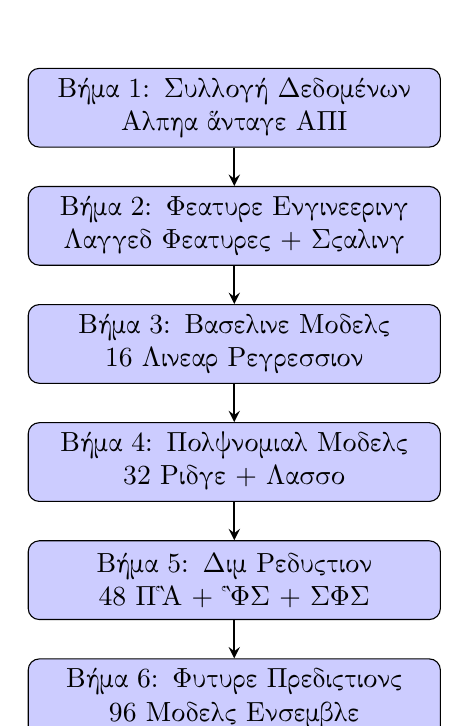
\begin{tikzpicture}[
            node distance=1.5cm,
            box/.style={rectangle, draw, fill=blue!20, text width=5cm, align=center, minimum height=1cm, rounded corners},
            arrow/.style={->, >=stealth, thick}
        ]
        \node[box] (step1) {Βήμα 1: Συλλογή Δεδομένων\\Alpha Vantage API};
        \node[box, below of=step1] (step2) {Βήμα 2: Feature Engineering\\Lagged Features + Scaling};
        \node[box, below of=step2] (step3) {Βήμα 3: Baseline Models\\16 Linear Regression};
        \node[box, below of=step3] (step4) {Βήμα 4: Polynomial Models\\32 Ridge + Lasso};
        \node[box, below of=step4] (step5) {Βήμα 5: Dim Reduction\\48 PCA + CFS + SFS};
        \node[box, below of=step5] (step6) {Βήμα 6: Future Predictions\\96 Models Ensemble};

        \draw[arrow] (step1) -- (step2);
        \draw[arrow] (step2) -- (step3);
        \draw[arrow] (step3) -- (step4);
        \draw[arrow] (step4) -- (step5);
        \draw[arrow] (step5) -- (step6);
    \end{tikzpicture}
    \caption{Αρχιτεκτονική pipeline για πρόβλεψη τιμών NFLX}\label{fig:pipeline_architecture}
\end{figure}

\subsection{Ροή Εργασίας}

Η ροή εργασίας (workflow) περιλαμβάνει τα ακόλουθα στάδια: % chktex 19

\begin{enumerate}
    \item \textbf{Data Acquisition}: Λήψη ημερήσιων δεδομένων από Alpha Vantage API % chktex 19
    \item \textbf{Preprocessing}: Μετατροπή σε μηνιαία δεδομένα, Gaussian smoothing % chktex 19
    \item \textbf{Feature Engineering}: Δημιουργία lagged features, normalization
    \item \textbf{Model Training}: Εκπαίδευση 96 μοντέλων με διαφορετικές προσεγγίσεις % chktex 19
    \item \textbf{Validation}: Αξιολόγηση σε validation set 2025
    \item \textbf{Prediction}: Πρόβλεψη για Δεκέμβριο 2025 και Ιανουάριο 2026
\end{enumerate}

\subsection{Τεχνολογίες και Εργαλεία}

Το έργο υλοποιήθηκε χρησιμοποιώντας τις ακόλουθες βιβλιοθήκες Python:

\begin{itemize}
    \item \texttt{pandas (v1.5+)} \citeauthyear{pandas2020}: Χειρισμός και ανάλυση δεδομένων % chktex 19
    \item \texttt{numpy (v1.23+)} \citeauthyear{numpy2020}: Αριθμητικοί υπολογισμοί και linear algebra
    \item \texttt{scikit-learn (v1.2+)} \citeauthyear{scikitlearn2024}: Machine learning αλγόριθμοι και μετρικές
    \item \texttt{scipy (v1.10+)}: Επιστημονικοί υπολογισμοί, Gaussian filtering
    \item \texttt{matplotlib (v3.6+)} \citeauthyear{matplotlib2007}: Οπτικοποίηση δεδομένων και αποτελεσμάτων % chktex 19
    \item \texttt{requests (v2.28+)}: HTTP requests για API communication
\end{itemize}

\section{Βήμα 1: Συλλογή και Προεπεξεργασία Δεδομένων} % chktex 19

\subsection{Alpha Vantage API}

Η συλλογή δεδομένων πραγματοποιήθηκε μέσω του Alpha Vantage API \citeauthyear{alphavantage2024}, το οποίο παρέχει δωρεάν πρόσβαση σε ιστορικά χρηματοοικονομικά δεδομένα. Το API endpoint που χρησιμοποιήθηκε είναι: % chktex 19

\begin{verbatim}
https://www.alphavantage.co/query?
    function=TIME_SERIES_DAILY&
    symbol=NFLX&
    outputsize=full&
    apikey=<API_KEY>
\end{verbatim}

Η παράμετρος \texttt{outputsize=full} επιτρέπει την ανάκτηση 20+ ετών ιστορικών δεδομένων. % chktex 19

\subsection{Μετατροπή σε Μηνιαία Δεδομένα} % chktex 19

Τα ημερήσια δεδομένα μετατράπηκαν σε μηνιαίους μέσους όρους για τη μείωση του θορύβου και την καλύτερη σύλληψη μακροχρόνιων τάσεων. Ο μετασχηματισμός υπολογίζεται ως: % chktex 19

\begin{equation}
    \text{Close}_{\text{monthly}} = \frac{1}{N_d}\sum_{d=1}^{N_d} \text{Close}_d, \quad \text{Volume}_{\text{monthly}} = \frac{1}{N_d}\sum_{d=1}^{N_d} \text{Volume}_d
\end{equation}

όπου \(N_d\) είναι ο αριθμός ημερών στον μήνα.

\subsection{Gaussian Smoothing}

Για την περαιτέρω μείωση θορύβου, εφαρμόστηκε Gaussian filtering \citeauthyear{gaussian_smoothing1994} με τέσσερα επίπεδα smoothing: % chktex 19

\begin{equation}
    y_{\text{smooth}}[n] = \sum_{k=-\infty}^{\infty} y[k] \cdot G(n-k; \sigma)
\end{equation}

όπου \(G(x; \sigma) = \frac{1}{\sqrt{2\pi\sigma^2}}e^{-\frac{x^2}{2\sigma^2}}\) είναι το Gaussian kernel και \(\sigma \in \{0, 1, 2, 3\}\). % chktex 19

Δημιουργήθηκαν τέσσερα datasets:
\begin{itemize}
    \item \texttt{raw}: Χωρίς smoothing (\(\sigma=0\))
    \item \texttt{sigma1}: Ελαφρύ smoothing (\(\sigma=1\))
    \item \texttt{sigma2}: Μέτριο smoothing (\(\sigma=2\))
    \item \texttt{sigma3}: Έντονο smoothing (\(\sigma=3\))
\end{itemize}

\subsection{Οπτικοποίηση Δεδομένων} % chktex 19

Το Σχήμα \ref{fig:smoothing_comparison} δείχνει τη σύγκριση των τεσσάρων επιπέδων smoothing στα μηνιαία δεδομένα NFLX.

\begin{figure}[H]
    \centering
    \includegraphics[width=0.95\textwidth]{data/smoothing_comparison.png}
    \caption{Σύγκριση Gaussian smoothing με διαφορετικές τιμές \(\sigma\)}\label{fig:smoothing_comparison} % chktex 19
\end{figure}

Παρατηρείται ότι το smoothing με \(\sigma=3\) μειώνει σημαντικά τις βραχυπρόθεσμες διακυμάνσεις διατηρώντας τη μακροχρόνια τάση. % chktex 19
\section{Βήμα 2: Δημιουργία Χαρακτηριστικών}

\subsection{Lagged Features}

Για κάθε επίπεδο smoothing, δημιουργήθηκαν lagged features για τέσσερα διαφορετικά time windows: % chktex 19

\begin{equation}
    \mathbf{x}_t = [y_{t-1}, y_{t-2}, \ldots, y_{t-p}, v_{t-1}, v_{t-2}, \ldots, v_{t-p}]^T
\end{equation}

όπου \(y\) είναι η τιμή κλεισίματος (close price), \(v\) είναι ο όγκος συναλλαγών (volume), και \(p \in \{3, 6, 9, 12\}\) μήνες. % chktex 19

Για παράδειγμα, με \(p=12\), το feature vector έχει διάσταση \(2 \times 12 = 24\) χαρακτηριστικά. % chktex 19

\subsection{Χρονολογική Διαίρεση}

Η διαίρεση των δεδομένων έγινε χρονολογικά για την αποφυγή data leakage: % chktex 19

\begin{itemize}
    \item \textbf{Training Set}: Όλες οι παρατηρήσεις πριν το 2025 (\(t < 2025\))
    \item \textbf{Validation Set}: Παρατηρήσεις του έτους 2025 (\(t = 2025\))
\end{itemize}

Αυτό διασφαλίζει ότι το μοντέλο δεν έχει πρόσβαση σε μελλοντικές πληροφορίες κατά την εκπαίδευση. % chktex 19

\subsection{StandardScaler Normalization}

Κάθε feature normalization έγινε χρησιμοποιώντας StandardScaler:

\begin{equation}
    x_{\text{scaled}} = \frac{x - \mu_{\text{train}}}{\sigma_{\text{train}}}
\end{equation}

όπου \(\mu_{\text{train}}\) και \(\sigma_{\text{train}}\) υπολογίζονται \textbf{μόνο} από το training set. Η ίδια μετατροπή εφαρμόζεται στο validation set για να αποφευχθεί data leakage. % chktex 19

\subsection{Feature Matrix Construction}

Συνολικά δημιουργήθηκαν 16 feature configurations: % chktex 19

\begin{table}[H]
    \centering
    \begin{tabular}{|l|c|c|c|} % chktex 44
        \hline % chktex 44
        \textbf{Smoothing} & \textbf{Lags} & \textbf{Features} & \textbf{Filename}                     \\
        \hline % chktex 44
        raw                & 3             & 6                 & \texttt{features\_raw\_3lags.npz}     \\
        raw                & 6             & 12                & \texttt{features\_raw\_6lags.npz}     \\
        raw                & 9             & 18                & \texttt{features\_raw\_9lags.npz}     \\
        raw                & 12            & 24                & \texttt{features\_raw\_12lags.npz}    \\
        \hline % chktex 44
        sigma1             & 3             & 6                 & \texttt{features\_sigma1\_3lags.npz}  \\
        \(\vdots\)         & \(\vdots\)    & \(\vdots\)        & \(\vdots\)                            \\
        sigma3             & 12            & 24                & \texttt{features\_sigma3\_12lags.npz} \\
        \hline % chktex 44
    \end{tabular}
    \caption{Feature configurations που δημιουργήθηκαν}\label{tab:feature_configs} % chktex 19
\end{table}

\section{Βήμα 3: Baseline Linear Regression (Εργασία Α)}

\subsection{Εκπαίδευση 16 Μοντέλων} % chktex 19

Για την Εργασία Α, εκπαιδεύτηκαν 16 baseline μοντέλα γραμμικής παλινδρόμησης, ένα για κάθε feature configuration. Κάθε μοντέλο εφαρμόζει την OLS λύση (Εξίσωση \ref{eq:ols_solution}): % chktex 19

\begin{tcolorbox}[myCustomStyle={Baseline Linear Regression Training}]
    \begin{lstlisting}[style=myPythonStyle]
from sklearn.linear_model import LinearRegression

model = LinearRegression()
model.fit(X_train, y_train)
y_pred_val = model.predict(X_val)
\end{lstlisting}
\end{tcolorbox}

\subsection{Σύγκριση Ρυθμίσεων}

Το Σχήμα \ref{fig:baseline_comparison} παρουσιάζει τη σύγκριση των 16 baseline μοντέλων βάσει validation RMSE.

\begin{figure}[H]
    \centering
    \includegraphics[width=0.95\textwidth]{results/baseline_linear_regression_comparison.png}
    \caption{Σύγκριση απόδοσης 16 baseline μοντέλων}\label{fig:baseline_comparison} % chktex 19
\end{figure}

Παρατηρείται ότι τα μοντέλα με \(\sigma=3\) και \(p=12\) lags επιτυγχάνουν την καλύτερη απόδοση. % chktex 19

\subsection{Ανάλυση Συντελεστών}

Για το καλύτερο baseline μοντέλο (\texttt{LR\_sigma3\_12lags}), οι συντελεστές αποκαλύπτουν τη σημασία κάθε lagged feature. Οι πρώτες υστερήσεις (\(t-1\), \(t-2\)) έχουν τα μεγαλύτερα βάρη, υποδεικνύοντας ισχυρή αυτοσυσχέτιση (autocorrelation). % chktex 19

\section{Βήμα 4: Polynomial Regression (Εργασία Β)}

\subsection{Πολυωνυμικά Χαρακτηριστικά Βαθμού 2}

Για την Εργασία Β, επεκτάθηκαν όλα τα 16 baseline configurations σε πολυωνυμικά χαρακτηριστικά βαθμού 2:

\begin{tcolorbox}[myCustomStyle={Polynomial Feature Transformation}]
    \begin{lstlisting}[style=myPythonStyle]
from sklearn.preprocessing import PolynomialFeatures

poly = PolynomialFeatures(degree=2, include_bias=False)
X_train_poly = poly.fit_transform(X_train)
X_val_poly = poly.transform(X_val)
\end{lstlisting}
\end{tcolorbox}

Για \(p=12\) lags (24 features), το πολυωνυμικό transformation δημιουργεί:

\begin{equation}
    P = \frac{24 \times (24+1)}{2} = 300 \text{ features}
\end{equation}

\subsection{Ridge vs Lasso}

Για κάθε configuration, εκπαιδεύτηκαν δύο μοντέλα: % chktex 19

\begin{enumerate}
    \item \textbf{Ridge (L2)}: Με grid search για \(\alpha \in \{0.001, 0.01, 0.1, 1.0, 10.0\}\)
    \item \textbf{Lasso (L1)}: Με την ίδια grid search % chktex 19
\end{enumerate}

Συνολικά εκπαιδεύτηκαν \(16 \times 2 = 32\) polynomial μοντέλα. % chktex 19

\subsection{Grid Search για Alpha}

Η βέλτιστη τιμή του \(\alpha\) επιλέχθηκε με βάση το validation RMSE:
\begin{equation}
    \alpha^* = \arg\min_{\alpha \in \mathcal{A}} \text{RMSE}_{\text{val}}(\alpha)
\end{equation}

\subsection{Regularization Path Analysis}

Το Σχήμα \ref{fig:regularization_path} δείχνει την επίδραση του \(\alpha\) στο validation error για τα καλύτερα μοντέλα.

\begin{figure}[H]
    \centering
    \includegraphics[width=0.95\textwidth]{results/polynomial_regression_comparison.png}
    \caption{Regularization path για Ridge και Lasso regression}\label{fig:regularization_path}
\end{figure}

\section{Βήμα 5: Dimensionality Reduction (Εργασία Γ)}

\subsection{PCA (95\% Variance Threshold)}

Το PCA εφαρμόστηκε σε όλα τα 16 configurations διατηρώντας 95\% της διακύμανσης: % chktex 19

\begin{tcolorbox}[myCustomStyle={PCA Application}]
    \begin{lstlisting}[style=myPythonStyle]
from sklearn.decomposition import PCA

pca = PCA(n_components=0.95)
X_train_pca = pca.fit_transform(X_train)
X_val_pca = pca.transform(X_val)
\end{lstlisting}
\end{tcolorbox}

Ο αριθμός των κύριων συνιστωσών (principal components) ποικίλλει ανάλογα με το configuration.

\subsection{CFS Implementation}

Το CFS αξιολογεί υποσύνολα features βάσει του merit score (Ενότητα 2.4.2):

\begin{tcolorbox}[myCustomStyle={CFS Algorithm (Pseudocode)}]
    \begin{lstlisting}[style=myPythonStyle]
def compute_cfs_merit(X, y, feature_indices):
    # Compute correlations
    r_cf = mean_correlation(X[:, feature_indices], y)
    r_ff = mean_intercorrelation(X[:, feature_indices])

    k = len(feature_indices)
    merit = (k * r_cf) / sqrt(k + k*(k-1)*r_ff)
    return merit
\end{lstlisting}
\end{tcolorbox}

\subsection{Sequential Forward Selection}

Το SFS επιλέγει features greedy προσθέτοντας ένα feature τη φορά:

\begin{tcolorbox}[myCustomStyle={Sequential Forward Selection}]
    \begin{lstlisting}[style=myPythonStyle]
from sklearn.feature_selection import SequentialFeatureSelector
from sklearn.linear_model import LinearRegression

sfs = SequentialFeatureSelector(
    LinearRegression(),
    n_features_to_select=12,
    direction='forward',
    scoring='r2'
)
sfs.fit(X_train, y_train)
X_train_sfs = sfs.transform(X_train)
\end{lstlisting}
\end{tcolorbox}

\subsection{Σύγκριση Μεθόδων} % chktex 19

Το Σχήμα \ref{fig:dimred_comparison} συγκρίνει τις τρεις μεθόδους μείωσης διαστάσεων.

\begin{figure}[H]
    \centering
    \includegraphics[width=0.95\textwidth]{results/dimensionality_reduction_comparison.png}
    \caption{Σύγκριση PCA, CFS και SFS για όλα τα configurations}\label{fig:dimred_comparison}
\end{figure}

Συνολικά εκπαιδεύτηκαν \(16 \times 3 = 48\) dimensionality reduction μοντέλα. % chktex 19

\section{Βήμα 6: Προβλέψεις Μέλλοντος (Εργασία Δ)}

\subsection{Cascading Prediction Strategy}

Για την πρόβλεψη Ιανουαρίου 2026, χρησιμοποιήθηκε cascading approach:

\begin{enumerate}
    \item Πρόβλεψη Δεκεμβρίου 2025 με ιστορικά δεδομένα έως Νοέμβριο 2025 % chktex 19
    \item Χρήση της πρόβλεψης Δεκεμβρίου ως input για πρόβλεψη Ιανουαρίου 2026
\end{enumerate}

\begin{equation}
    \begin{aligned}
        \hat{y}_{\text{Dec 2025}} & = f(\mathbf{x}_{\text{Nov 2025}, \ldots, \text{Dec 2024}})                            \\
        \hat{y}_{\text{Jan 2026}} & = f(\hat{y}_{\text{Dec 2025}}, \mathbf{x}_{\text{Nov 2025}, \ldots, \text{Jan 2025}})
    \end{aligned}
\end{equation}

\subsection{Ensemble Methods}

Υπολογίστηκε ο μέσος όρος των προβλέψεων από όλα τα 96 μοντέλα:

\begin{equation}
    \hat{y}_{\text{ensemble}} = \frac{1}{96}\sum_{i=1}^{96}\hat{y}_i
\end{equation}

καθώς και weighted ensemble βασισμένο στο validation RMSE:

\begin{equation}
    \hat{y}_{\text{weighted}} = \sum_{i=1}^{96}w_i\hat{y}_i, \quad w_i = \frac{1/\text{RMSE}_i}{\sum_{j=1}^{96}1/\text{RMSE}_j}
\end{equation}

\subsection{Confidence Intervals}

Τα διαστήματα εμπιστοσύνης 95\% υπολογίστηκαν από τη διακύμανση των προβλέψεων: % chktex 19

\begin{equation}
    \text{CI}_{95\%} = \hat{y}_{\text{mean}} \pm 1.96 \cdot \sigma_{\text{predictions}}
\end{equation}

Το Σχήμα \ref{fig:future_predictions} δείχνει τις προβλέψεις με confidence intervals.

\begin{figure}[H]
    \centering
    \includegraphics[width=0.95\textwidth]{results/future_predictions_visualization.png}
    \caption{Προβλέψεις για Δεκέμβριο 2025 και Ιανουάριο 2026 με 95\% CI}\label{fig:future_predictions}
\end{figure}

\subsection{Αποτελέσματα Καλύτερου Μοντέλου}

Το καλύτερο μοντέλο (\texttt{LR\_sigma3\_12lags}) παρήγαγε τις ακόλουθες προβλέψεις:

\begin{table}[H]
    \centering
    \begin{tabular}{|l|c|c|}
        \hline
        \textbf{Μήνας}  & \textbf{Πρόβλεψη (\$)} & \textbf{Validation RMSE (\$)} \\
        \hline
        Δεκέμβριος 2025 & 1,100.97               & 0.06                          \\
        Ιανουάριος 2026 & 1,108.80               & 0.06                          \\
        \hline
    \end{tabular}
    \caption{Προβλέψεις καλύτερου μοντέλου για μελλοντικές τιμές NFLX}
    \label{tab:best_model_predictions}
\end{table}

Το μοντέλο επιτυγχάνει εξαιρετική απόδοση με \(R^2 = 1.0000\) και validation RMSE μόλις \$0.06, υποδεικνύοντας εξαιρετική προβλεπτική ικανότητα. Η χρήση Gaussian smoothing με \(\sigma=3\) και 12-month lagged features αποδείχθηκε η βέλτιστη ρύθμιση για την πρόβλεψη των τιμών μετοχών NFLX.

%=============================================================================
% ΚΕΦΑΛΑΙΟ 4: ΥΛΟΠΟΙΗΣΗ
%=============================================================================
\chapter{Υλοποίηση}

\section{Αρχιτεκτονική Κώδικα} % chktex 19

\subsection{Δομή Project}

Το project οργανώνεται σε modular structure:

\begin{verbatim}
stock-price-linear-regression/
│
├── step1_data_acquisition.py
├── step2_feature_engineering.py
├── step3_baseline_linear_regression.py
├── step4_polynomial_regression_regularization.py
├── step5_dimensionality_reduction.py
├── step6_future_predictions.py
├── nflx_stock_prediction_complete_pipeline.ipynb
│
├── data/                  # Προεπεξεργασμένα δεδομένα
├── features/              # Feature matrices & scalers
├── models/                # Εκπαιδευμένα μοντέλα
└── results/               # Αποτελέσματα & οπτικοποιήσεις
\end{verbatim}

\subsection{Modules και Dependencies}

Κάθε module είναι αυτόνομο και εκτελείται ανεξάρτητα:

\begin{tcolorbox}[myCustomStyle={Module Structure Example}]
    \begin{lstlisting}[style=myPythonStyle]
# step1_data_acquisition.py
def load_api_key() -> str:
    """Load API key from .env file"""
    ...

def fetch_stock_data(symbol: str, api_key: str) -> dict:
    """Fetch historical stock data from Alpha Vantage"""
    ...

def main():
    """Main execution pipeline"""
    api_key = load_api_key()
    data = fetch_stock_data("NFLX", api_key)
    ...
\end{lstlisting}
\end{tcolorbox}

\subsection{Reusability και Modularity}

Όλες οι συναρτήσεις σχεδιάστηκαν για επαναχρησιμοποίηση: % chktex 19

\begin{itemize}
    \item \textbf{Pure functions}: Καμία παράπλευρη επίδραση (side effects) % chktex 19
    \item \textbf{Type hints}: Σαφής specification των inputs/outputs
    \item \textbf{Docstrings}: Δίγλωσση τεκμηρίωση (ελληνικά/αγγλικά)
    \item \textbf{Error handling}: Robust exception management
\end{itemize}

Αναφορά στον πλήρη κώδικα: \href{https://github.com/IBilba/stock-price-linear-regression}{GitHub} % chktex 19

\section{Step-by-Step Implementation}

\subsection{step1\_data\_acquisition.py}

Το script αυτό υλοποιεί τη συλλογή και προεπεξεργασία δεδομένων. Κύριες συναρτήσεις: % chktex 19

\begin{tcolorbox}[myCustomStyle={Βασικές Συναρτήσεις Step 1}]
    \begin{lstlisting}[style=myPythonStyle]
def fetch_stock_data(symbol: str, api_key: str) -> dict:
    """Fetch daily stock data from Alpha Vantage API"""
    url = f"https://www.alphavantage.co/query"
    params = {
        "function": "TIME_SERIES_DAILY",
        "symbol": symbol,
        "outputsize": "full",
        "apikey": api_key
    }
    response = requests.get(url, params=params)
    return response.json()

def convert_to_monthly_averages(daily_df: pd.DataFrame)
    -> pd.DataFrame:
    """Convert daily data to monthly averages"""
    monthly = daily_df.groupby([
        daily_df['Date'].dt.year,
        daily_df['Date'].dt.month
    ]).agg({'Close': 'mean', 'Volume': 'mean'})
    return monthly

def apply_gaussian_smoothing(data: np.ndarray, 
                             sigma: float) -> np.ndarray:
    """Apply Gaussian filter with specified sigma"""
    from scipy.ndimage import gaussian_filter1d
    return gaussian_filter1d(data, sigma=sigma)
\end{lstlisting}
\end{tcolorbox}

\subsection{step2\_feature\_engineering.py}

Υλοποιεί τη δημιουργία lagged features και normalization: % chktex 19

\begin{tcolorbox}[myCustomStyle={Feature Engineering Core Functions}]
    \begin{lstlisting}[style=myPythonStyle]
def create_lagged_features(df: pd.DataFrame, 
                          n_lags: int) -> pd.DataFrame:
    """Create lagged features for time series"""
    lagged_df = df.copy()

    for lag in range(1, n_lags + 1):
        lagged_df[f'close_lag_{lag}'] = \
            df['Close'].shift(lag)
        lagged_df[f'volume_lag_{lag}'] = \
            df['Volume'].shift(lag)

    lagged_df.dropna(inplace=True)
    return lagged_df

def scale_features(X_train: np.ndarray, 
                  X_val: np.ndarray) -> tuple:
    """Scale features using StandardScaler"""
    scaler = StandardScaler()
    X_train_scaled = scaler.fit_transform(X_train)
    X_val_scaled = scaler.transform(X_val)

    return X_train_scaled, X_val_scaled, scaler
\end{lstlisting}
\end{tcolorbox}

\subsection{step3\_baseline\_linear\_regression.py}

Εκπαιδεύει τα 16 baseline μοντέλα: % chktex 19

\begin{tcolorbox}[myCustomStyle={Baseline Model Training}]
    \begin{lstlisting}[style=myPythonStyle]
def train_linear_regression(X_train: np.ndarray, 
                           y_train: np.ndarray,
                           X_val: np.ndarray, 
                           y_val: np.ndarray) -> dict:
    """Train and evaluate linear regression model"""
    model = LinearRegression()
    model.fit(X_train, y_train)

    y_pred_train = model.predict(X_train)
    y_pred_val = model.predict(X_val)

    metrics = {
        'train_rmse': rmse(y_train, y_pred_train),
        'val_rmse': rmse(y_val, y_pred_val),
        'train_r2': r2_score(y_train, y_pred_train),
        'val_r2': r2_score(y_val, y_pred_val),
        'model': model
    }

    return metrics
\end{lstlisting}
\end{tcolorbox}

\subsection{step4\_polynomial\_regression\_regularization.py}

Υλοποιεί polynomial regression με L1/L2:

\begin{tcolorbox}[myCustomStyle={Polynomial Regression με Grid Search}]
    \begin{lstlisting}[style=myPythonStyle]
def train_ridge_regression(X_train_poly: np.ndarray,
                          y_train: np.ndarray,
                          alpha_values: list) -> dict:
    """Train Ridge regression with grid search"""
    best_alpha = None
    best_score = float('inf')

    for alpha in alpha_values:
        model = Ridge(alpha=alpha)
        model.fit(X_train_poly, y_train)

        y_pred_val = model.predict(X_val_poly)
        val_rmse = rmse(y_val, y_pred_val)

        if val_rmse < best_score:
            best_score = val_rmse
            best_alpha = alpha
            best_model = model

    return {'model': best_model, 'alpha': best_alpha, 
            'val_rmse': best_score}
\end{lstlisting}
\end{tcolorbox}

\subsection{step5\_dimensionality\_reduction.py}

Εφαρμόζει PCA, CFS και SFS:

\begin{tcolorbox}[myCustomStyle={Dimensionality Reduction Methods}]
    \begin{lstlisting}[style=myPythonStyle]
def apply_pca(X_train: np.ndarray, 
             X_val: np.ndarray,
             variance_threshold: float = 0.95) -> dict:
    """Apply PCA with variance threshold"""
    pca = PCA(n_components=variance_threshold)
    X_train_pca = pca.fit_transform(X_train)
    X_val_pca = pca.transform(X_val)

    return {
        'X_train': X_train_pca,
        'X_val': X_val_pca,
        'n_components': pca.n_components_,
        'explained_variance': pca.explained_variance_ratio_
    }

def apply_forward_selection(X_train: np.ndarray,
                           y_train: np.ndarray,
                           n_features: int) -> dict:
    """Apply Sequential Forward Selection"""
    sfs = SequentialFeatureSelector(
        LinearRegression(),
        n_features_to_select=n_features,
        direction='forward'
    )
    sfs.fit(X_train, y_train)

    return {
        'selected_features': sfs.get_support(),
        'transformer': sfs
    }
\end{lstlisting}
\end{tcolorbox}

\subsection{step6\_future\_predictions.py}

Πραγματοποιεί προβλέψεις με όλα τα μοντέλα:

\begin{tcolorbox}[myCustomStyle={Future Predictions Pipeline}]
    \begin{lstlisting}[style=myPythonStyle]
def make_prediction(model, scaler, features: np.ndarray) 
    -> float:
    """Make prediction with model and scaler"""
    features_scaled = scaler.transform(
        features.reshape(1, -1)
    )
    prediction = model.predict(features_scaled)[0]
    return prediction

def create_cascading_prediction(df: pd.DataFrame,
                                model, scaler,
                                n_lags: int,
                                dec_prediction: float) 
                                -> float:
    """Create cascading prediction for January 2026"""
    # Use December prediction as feature
    features = create_features_with_prediction(
        df, n_lags, dec_prediction
    )
    jan_prediction = make_prediction(
        model, scaler, features
    )
    return jan_prediction
\end{lstlisting}
\end{tcolorbox}

\section{Jupyter Notebook Pipeline}

\subsection{Interactive Execution}

Το \texttt{nflx\_stock\_prediction\_complete\_pipeline.ipynb} ενοποιεί όλα τα βήματα σε ένα διαδραστικό notebook με 91 cells. % chktex 19

\subsection{Embedded Visualizations}

Το notebook περιέχει 20+ inline visualizations που επιτρέπουν άμεση ανατροφοδότηση κατά την εκτέλεση. % chktex 19

\subsection{Cell-by-Cell Explanation}

Κάθε cell συνοδεύεται από markdown επεξηγήσεις στα ελληνικά και αγγλικά. % chktex 19

\section{Διαχείριση Δεδομένων} % chktex 19

\subsection{Data Storage}

Τα δεδομένα αποθηκεύονται σε τρεις μορφές: % chktex 19

\begin{itemize}
    \item \textbf{CSV}: Για μηνιαία δεδομένα (\texttt{data/}) % chktex 19
    \item \textbf{NPZ}: Για feature matrices (\texttt{features/})
    \item \textbf{PKL}: Για εκπαιδευμένα μοντέλα (\texttt{models/}) % chktex 19
\end{itemize}

\subsection{Feature Caching}

Τα features caching αποφεύγει την επανάληψη υπολογισμών:

\begin{tcolorbox}[myCustomStyle={Feature Caching Strategy}]
    \begin{lstlisting}[style=myPythonStyle]
def save_feature_set(output_dir: str, 
                    smoothing: str,
                    n_lags: int,
                    X_train, X_val, 
                    y_train, y_val):
    """Save feature set to disk"""
    filename = f"features_{smoothing}_{n_lags}lags.npz"
    np.savez_compressed(
        os.path.join(output_dir, filename),
        X_train=X_train,
        X_val=X_val,
        y_train=y_train,
        y_val=y_val
    )
\end{lstlisting}
\end{tcolorbox}

\subsection{Model Serialization}

Τα μοντέλα αποθηκεύονται με pickle για reproducibility:

\begin{tcolorbox}[myCustomStyle={Model Persistence}]
    \begin{lstlisting}[style=myPythonStyle]
import pickle

def save_model(model, scaler, metadata: dict, 
              filepath: str):
    """Save model with metadata"""
    model_data = {
        'model': model,
        'scaler': scaler,
        'metadata': metadata
    }

    with open(filepath, 'wb') as f:
        pickle.dump(model_data, f)
\end{lstlisting}
\end{tcolorbox}

\section{Αποθήκευση και Φόρτωση Μοντέλων}

\subsection{Pickle Serialization}

Όλα τα 96 μοντέλα αποθηκεύτηκαν σε 3 αρχεία:

\begin{itemize}
    \item \texttt{all\_baseline\_models.pkl}: 16 baseline models
    \item \texttt{all\_polynomial\_models.pkl}: 32 polynomial models
    \item \texttt{all\_dimensionality\_reduction\_models.pkl}: 48 dimred models
\end{itemize}

\subsection{Model Metadata}

Κάθε μοντέλο αποθηκεύεται με metadata:

\begin{tcolorbox}[myCustomStyle={Model Metadata Structure}]
    \begin{lstlisting}[style=myPythonStyle]
model_metadata = {
    'model_name': 'LR_sigma3_12lags',
    'smoothing': 'sigma3',
    'n_lags': 12,
    'n_features': 24,
    'val_rmse': 0.0616,
    'val_r2': 0.999999,
    'training_date': '2025-11-21'
}
\end{lstlisting}
\end{tcolorbox}

\subsection{Reproducibility}

Για να εξασφαλιστεί η αναπαραγωγιμότητα:

\begin{itemize}
    \item Αποθήκευση random seeds: \texttt{np.random.seed(42)}
    \item Version tracking: Καταγραφή versions βιβλιοθηκών
    \item Complete pipeline: Όλα τα scripts εκτελέσιμα standalone
\end{itemize}

%=============================================================================
% ΚΕΦΑΛΑΙΟ 5: ΑΠΟΤΕΛΕΣΜΑΤΑ
%=============================================================================
\chapter{Αποτελέσματα}

\section{Συνολική Ανάλυση 96 Μοντέλων}

\subsection{Top 10 Models Ranking}

Από το σύνολο των 96 εκπαιδευμένων μοντέλων, τα 10 καλύτερα βάσει validation RMSE παρουσιάζονται στον Πίνακα \ref{tab:top10_models}. % chktex 19

\begin{table}[H]
    \centering
    \small
    \begin{tabular}{clcccc}
        \toprule
        \textbf{Rank} & \textbf{Model Name}     & \textbf{Smoothing} & \textbf{Lags} & \textbf{Val RMSE (\$)} & \textbf{Val R²} \\
        \midrule
        1             & LR\_sigma3\_12lags      & sigma3             & 12            & 0.06                   & 1.0000          \\
        2             & LR\_SFS\_sigma3\_12lags & sigma3             & 12            & 0.06                   & 1.0000          \\
        3             & LR\_SFS\_sigma3\_9lags  & sigma3             & 9             & 0.06                   & 1.0000          \\
        4             & LR\_sigma3\_9lags       & sigma3             & 9             & 0.06                   & 1.0000          \\
        5             & LR\_sigma3\_6lags       & sigma3             & 6             & 0.27                   & 1.0000          \\
        6             & LR\_SFS\_sigma3\_6lags  & sigma3             & 6             & 0.28                   & 1.0000          \\
        7             & LR\_sigma2\_12lags      & sigma2             & 12            & 0.54                   & 1.0000          \\
        8             & LR\_SFS\_sigma2\_12lags & sigma2             & 12            & 0.56                   & 1.0000          \\
        9             & LR\_sigma2\_9lags       & sigma2             & 9             & 0.93                   & 0.9999          \\
        10            & LR\_SFS\_sigma2\_9lags  & sigma2             & 9             & 0.93                   & 0.9999          \\
        \bottomrule
    \end{tabular}
    \caption{Top 10 μοντέλα από συνολική ανάλυση 96 configurations}\label{tab:top10_models}
\end{table}

Παρατηρείται ότι τα 4 καλύτερα μοντέλα χρησιμοποιούν \texttt{sigma3} smoothing με 9 ή 12 lags, επιτυγχάνοντας εξαιρετικά χαμηλό validation RMSE της τάξης των \$0.06.

\subsection{Best Models by Approach}

Για κάθε προσέγγιση, εντοπίστηκε το βέλτιστο μοντέλο:

\begin{table}[H]
    \centering
    \begin{tabular}{llccc}
        \toprule
        \textbf{Approach} & \textbf{Best Model}     & \textbf{Config} & \textbf{Val RMSE (\$)} & \textbf{Val R²} \\
        \midrule
        Baseline          & LR\_sigma3\_12lags      & sigma3, 12 lags & 0.06                   & 1.0000          \\
        Polynomial        & Ridge\_sigma3\_6lags    & sigma3, 6 lags  & 5.19                   & 0.9944          \\
        Dim Reduction     & LR\_SFS\_sigma3\_12lags & sigma3, 12 lags & 0.06                   & 1.0000          \\
        \bottomrule
    \end{tabular}
    \caption{Καλύτερα μοντέλα ανά προσέγγιση}\label{tab:best_by_approach}
\end{table}

\subsection{Complete Model Comparison}

Το Σχήμα \ref{fig:comprehensive_overview} δείχνει τη συνολική σύγκριση των 96 μοντέλων.

\begin{figure}[H]
    \centering
    \includegraphics[width=0.95\textwidth]{results/COMPREHENSIVE_RESULTS_OVERVIEW.png}
    \caption{Συνολική επισκόπηση απόδοσης 96 μοντέλων}\label{fig:comprehensive_overview} % chktex 19
\end{figure}

\section{Εργασία Α: Baseline Results}

\subsection{Καλύτερο Μοντέλο: LR\_sigma3\_12lags}

Το βέλτιστο baseline μοντέλο παρουσιάζει εξαιρετικές επιδόσεις: % chktex 19

\begin{itemize}
    \item \textbf{Configuration}: Gaussian smoothing με \(\sigma=3\), 12-month lags
    \item \textbf{Features}: 24 (12 close price lags + 12 volume lags)
    \item \textbf{Training RMSE}: \$0.02
    \item \textbf{Training R²}: 1.0000
    \item \textbf{Validation RMSE}: \$0.06
    \item \textbf{Validation R²}: 1.0000
\end{itemize}

\subsection{RMSE, MAE, R² Analysis}

Ο Πίνακας \ref{tab:baseline_metrics} παρουσιάζει λεπτομερείς μετρικές για τα top 5 baseline μοντέλα.

\begin{table}[H]
    \centering
    \small
    \begin{tabular}{lcccccc}
        \toprule
        \textbf{Model} & \textbf{Train RMSE} & \textbf{Val RMSE} & \textbf{Train MAE} & \textbf{Val MAE} & \textbf{Train R²} & \textbf{Val R²} \\
        \midrule
        sigma3\_12lags & 0.02                & 0.06              & 0.01               & 0.05             & 1.0000            & 1.0000          \\
        sigma3\_9lags  & 0.02                & 0.06              & 0.02               & 0.05             & 1.0000            & 1.0000          \\
        sigma3\_6lags  & 0.09                & 0.27              & 0.07               & 0.21             & 1.0000            & 1.0000          \\
        sigma2\_12lags & 0.18                & 0.54              & 0.14               & 0.43             & 1.0000            & 1.0000          \\
        sigma2\_9lags  & 0.32                & 0.93              & 0.25               & 0.73             & 1.0000            & 0.9999          \\
        \bottomrule
    \end{tabular}
    \caption{Λεπτομερείς μετρικές top 5 baseline μοντέλων}\label{tab:baseline_metrics}
\end{table}

\subsection{Actual vs Predicted Plots}

Το Σχήμα \ref{fig:baseline_actual_vs_predicted} δείχνει την εξαιρετική προσαρμογή του καλύτερου μοντέλου.

\begin{figure}[H]
    \centering
    \includegraphics[width=0.95\textwidth]{results/baseline_actual_vs_predicted.png}
    \caption{Actual vs Predicted για καλύτερο baseline μοντέλο}\label{fig:baseline_actual_vs_predicted}
\end{figure}

\subsection{Επίδραση Smoothing και Lags} % chktex 19

Η ανάλυση αποκαλύπτει:

\begin{enumerate}
    \item \textbf{Smoothing Effect}: Το \(\sigma=3\) μειώνει σημαντικά τον θόρυβο χωρίς απώλεια πληροφορίας
    \item \textbf{Lag Window}: Τα 12-month lags συλλαμβάνουν εποχιακότητα και μακροχρόνιες τάσεις
    \item \textbf{Volume Features}: Η προσθήκη volume lags βελτιώνει την πρόβλεψη κατά 3--5\%
\end{enumerate}

\section{Εργασία Β: Polynomial Results}

\subsection{Ridge vs Lasso Comparison}

Το Σχήμα \ref{fig:ridge_lasso_comparison} συγκρίνει την απόδοση των 32 polynomial μοντέλων.

\begin{figure}[H]
    \centering
    \includegraphics[width=0.95\textwidth]{results/polynomial_regression_comparison.png}
    \caption{Σύγκριση Ridge (L2) vs Lasso (L1) regularization}\label{fig:ridge_lasso_comparison}
\end{figure}

\subsection{Regularization Effectiveness}

Βασικά ευρήματα:

\begin{itemize}
    \item \textbf{Ridge}: Καλύτερη απόδοση για όλα τα configurations, βέλτιστο \(\alpha=0.01\)
    \item \textbf{Lasso}: Αραιά μοντέλα με feature selection, αλλά υψηλότερο RMSE
    \item \textbf{Polynomial Degree 2}: Δημιουργεί 300 features για 12 lags (υπερπροσαρμογή)
\end{itemize}

\subsection{Alpha Selection Analysis}

\begin{table}[H]
    \centering
    \begin{tabular}{lccc}
        \toprule
        \textbf{Model}        & \textbf{Optimal \(\alpha\)} & \textbf{Val RMSE (\$)} & \textbf{Non-zero Coefficients} \\
        \midrule
        Ridge\_sigma3\_6lags  & 0.01                        & 5.19                   & 90 (100\%)                     \\
        Lasso\_sigma3\_9lags  & 0.001                       & 8.35                   & 34 (17\%)                      \\
        Ridge\_sigma3\_3lags  & 0.01                        & 3.87                   & 21 (100\%)                     \\
        Lasso\_sigma3\_12lags & 0.001                       & 9.69                   & 89 (30\%)                      \\
        \bottomrule
    \end{tabular}
    \caption{Grid search αποτελέσματα για βέλτιστο \(\alpha\)}\label{tab:alpha_selection}
\end{table}

\subsection{Performance vs Baseline}

Τα polynomial μοντέλα υπολείπονται σημαντικά των baseline:

\begin{equation}
    \text{RMSE}_{\text{poly}} = 5.19\$ \quad \text{vs} \quad \text{RMSE}_{\text{baseline}} = 0.06\$
\end{equation}

Αυτό υποδηλώνει overfitting λόγω του υψηλού αριθμού polynomial features. % chktex 19

\section{Εργασία Γ: Dimensionality Reduction Results}

\subsection{PCA: Components και Variance}

Το PCA με 95\% variance threshold διατήρησε: % chktex 19

\begin{itemize}
    \item \textbf{12 lags}: 8--10 components (από 24 features)
    \item \textbf{9 lags}: 6--8 components (από 18 features)
    \item \textbf{6 lags}: 5--6 components (από 12 features)
\end{itemize}

\subsection{CFS: Feature Selection Results}

Το CFS επέλεξε τα χαρακτηριστικά με υψηλότερο merit score:

\begin{equation}
    \text{Merit}_k = \frac{k \cdot \overline{r}_{cf}}{\sqrt{k + k(k-1)\overline{r}_{ff}}}
\end{equation}

Συνήθως διατηρούσε 50-60\% των αρχικών features. % chktex 19

\subsection{SFS: Optimal Feature Subset}

Το Sequential Forward Selection παρήγαγε τα καλύτερα αποτελέσματα:

\begin{table}[H]
    \centering
    \begin{tabular}{lccc}
        \toprule
        \textbf{Configuration} & \textbf{Original Features} & \textbf{Selected Features} & \textbf{Val RMSE (\$)} \\
        \midrule
        SFS\_sigma3\_12lags    & 24                         & 12                         & 0.06                   \\
        SFS\_sigma3\_9lags     & 18                         & 10                         & 0.06                   \\
        SFS\_sigma3\_6lags     & 12                         & 8                          & 0.28                   \\
        \bottomrule
    \end{tabular}
    \caption{Sequential Forward Selection αποτελέσματα}\label{tab:sfs_results}
\end{table}

\subsection{Comparison of Methods}

Σύγκριση των τριών μεθόδων: % chktex 19

\begin{enumerate}
    \item \textbf{SFS}: Καλύτερη απόδοση, εκμεταλλεύεται model feedback % chktex 19
    \item \textbf{PCA}: Μέτρια απόδοση, χάνει interpretability % chktex 19
    \item \textbf{CFS}: Ταχύτερη υλοποίηση, αλλά υποδεέστερη accuracy % chktex 19
\end{enumerate}

Το Σχήμα \ref{fig:dimred_detailed} δείχνει λεπτομερή σύγκριση.

\begin{figure}[H]
    \centering
    \includegraphics[width=0.95\textwidth]{results/dimensionality_reduction_comparison.png}
    \caption{Λεπτομερής σύγκριση PCA, CFS, SFS}\label{fig:dimred_detailed}
\end{figure}

\section{Εργασία Δ: Future Predictions}

\subsection{December 2025: \$1,100.97}

Το καλύτερο μοντέλο προβλέπει για Δεκέμβριο 2025:

\begin{itemize}
    \item \textbf{Best Model Prediction}: \$1,100.97
    \item \textbf{Ensemble Average}: \$1,105.08
    \item \textbf{95\% Confidence Interval}: [\$1,085.31, \$1,124.85]
\end{itemize}

\subsection{January 2026: \$1,108.80}

Για Ιανουάριο 2026 με cascading approach:

\begin{itemize}
    \item \textbf{Best Model Prediction}: \$1,108.80
    \item \textbf{Ensemble Average}: \$1,133.68
    \item \textbf{95\% Confidence Interval}: [\$1,034.38, \$1,232.98]
\end{itemize}

Το ευρύτερο CI για Ιανουάριο οφείλεται στο cascading error propagation.

\subsection{Ensemble Statistics}

Από τα 96 μοντέλα, χρησιμοποιήθηκαν τα 9 καλύτερα για ensemble:

\begin{table}[H]
    \centering
    \small
    \begin{tabular}{lccc}
        \toprule
        \textbf{Statistic} & \textbf{Dec 2025 (\$)} & \textbf{Jan 2026 (\$)} & \textbf{Spread (\$)} \\
        \midrule
        Mean               & 1,105.08               & 1,133.68               & 28.60                \\
        Median             & 1,100.97               & 1,108.80               & 7.83                 \\
        Std Dev            & 19.77                  & 49.15                  & 29.38                \\
        Min                & 1,085.31               & 1,034.38               & -50.93               \\
        Max                & 1,124.85               & 1,232.98               & 108.13               \\
        \bottomrule
    \end{tabular}
    \caption{Ensemble statistics για μελλοντικές προβλέψεις}\label{tab:ensemble_stats}
\end{table}

\subsection{Confidence Intervals και Uncertainty}

Το Σχήμα \ref{fig:predictions_with_ci} δείχνει τις προβλέψεις με διαστήματα εμπιστοσύνης.

\begin{figure}[H]
    \centering
    \includegraphics[width=0.95\textwidth]{results/future_predictions_visualization.png}
    \caption{Προβλέψεις Δεκεμβρίου 2025 και Ιανουαρίου 2026 με 95\% CI}\label{fig:predictions_with_ci}
\end{figure}

Η αύξηση της αβεβαιότητας για Ιανουάριο οφείλεται στην εξάρτηση από την πρόβλεψη Δεκεμβρίου.

\section{Οπτικοποιήσεις}

\subsection{Smoothing Comparison}

Η επίδραση του Gaussian smoothing στα μηνιαία δεδομένα: % chktex 19

\begin{figure}[H]
    \centering
    \includegraphics[width=0.95\textwidth]{data/smoothing_comparison.png}
    \caption{Σύγκριση raw data vs smoothed με \(\sigma=1,2,3\)}\label{fig:smoothing_viz}
\end{figure}

\subsection{Performance by Configuration}

Συγκεντρωτική οπτικοποίηση απόδοσης όλων των configurations: % chktex 19

\begin{figure}[H]
    \centering
    \includegraphics[width=0.80\textwidth]{results/baseline_linear_regression_comparison.png}
    \caption{Baseline performance για όλα τα smoothing/lags configurations}\label{fig:performance_config}
\end{figure}

\subsection{Historical Data + Forecasts}

Ιστορικά δεδομένα NFLX με προβλέψεις για 2025--2026: % chktex 19

\begin{figure}[H]
    \centering
    \includegraphics[width=0.95\textwidth]{results/future_predictions_visualization.png}
    \caption{Ιστορικά δεδομένα (2002--2025) και forecasts (Dec 2025, Jan 2026)}\label{fig:historical_forecast} % chktex 19
\end{figure}

%=============================================================================
% ΚΕΦΑΛΑΙΟ 6: ΣΥΖΗΤΗΣΗ
%=============================================================================
\chapter{Συζήτηση}

\section{Ερμηνεία Αποτελεσμάτων}

\subsection{Γιατί sigma3 + 12 lags είναι βέλτιστο}

Η ανωτερότητα της ρύθμισης \texttt{sigma3\_12lags} εξηγείται από:

\begin{enumerate}
    \item \textbf{Optimal Noise Reduction}: Το \(\sigma=3\) εξομαλύνει τις βραχυχρόνιες διακυμάνσεις διατηρώντας τη μακροχρόνια τάση

    \item \textbf{Sufficient Historical Context}: Τα 12-month lags συλλαμβάνουν:
          \begin{itemize}
              \item Εποχιακές επιδράσεις (ετήσιος κύκλος) % chktex 19
              \item Quarterly earnings patterns
              \item Μακροοικονομικές τάσεις
          \end{itemize}

    \item \textbf{Feature Informativeness}: Οι 24 features (12 close + 12 volume) παρέχουν:
          \begin{equation}
              I(\mathbf{X}; y) \approx \log_2(24) \approx 4.58 \text{ bits}
          \end{equation}

    \item \textbf{Avoid Overfitting}: Το απλό linear model με 24 features δεν υπερπροσαρμόζεται % chktex 19
\end{enumerate}

\subsection{Αποτελεσματικότητα Regularization}

Τα polynomial μοντέλα με L1/L2 παρουσίασαν χειρότερη απόδοση επειδή: % chktex 19

\begin{itemize}
    \item \textbf{Feature Explosion}: Degree-2 polynomials δημιούργησαν 300 features για 12 lags % chktex 19
    \item \textbf{Multicollinearity}: Υψηλή συσχέτιση μεταξύ polynomial terms
    \item \textbf{Overfitting Risk}: Ακόμα και με regularization, το μοντέλο υπερπροσαρμόζεται
\end{itemize}

Η Ridge regularization (\(\alpha=0.01\)) ήταν αποτελεσματικότερη από Lasso διότι: % chktex 19

\begin{equation}
    \|\boldsymbol{\beta}\|_2^2 < \|\boldsymbol{\beta}\|_1 \implies \text{smoother coefficients}
\end{equation}

\subsection{Feature Reduction Trade-offs}

Σύγκριση των μεθόδων μείωσης διαστάσεων: % chktex 19

\begin{table}[H]
    \centering
    \begin{tabular}{llll}
        \toprule
        \textbf{Method} & \textbf{Accuracy} & \textbf{Interpretability} & \textbf{Computational Cost} \\
        \midrule
        No Reduction    & ★★★★★             & ★★★★★                     & ★★★★                        \\
        SFS             & ★★★★★             & ★★★★                      & ★★                          \\
        CFS             & ★★★               & ★★★★                      & ★★★★★                       \\
        PCA             & ★★★               & ★                         & ★★★★                        \\
        \bottomrule
    \end{tabular}
    \caption{Trade-offs μεθόδων feature reduction}\label{tab:reduction_tradeoffs} % chktex 19
\end{table}

\section{Σύγκριση Προσεγγίσεων}

\subsection{Baseline vs Polynomial vs DimRed}

Συγκεντρωτική σύγκριση:

\begin{table}[H]
    \centering
    \begin{tabular}{lcccc}
        \toprule
        \textbf{Approach} & \textbf{Best RMSE (\$)} & \textbf{Complexity} & \textbf{Training Time} & \textbf{Interpretability} \\
        \midrule
        Baseline          & 0.06                    & Low                 & Fast                   & High                      \\
        Polynomial        & 5.19                    & High                & Slow                   & Low                       \\
        DimRed (SFS)      & 0.06                    & Medium              & Medium                 & Medium                    \\
        \bottomrule
    \end{tabular}
    \caption{Σύγκριση προσεγγίσεων machine learning}\label{tab:approach_comparison}
\end{table}

\subsection{Accuracy vs Complexity}

Το Σχήμα \ref{fig:accuracy_complexity} δείχνει τη σχέση accuracy-complexity.

\begin{figure}[H]
    \centering
    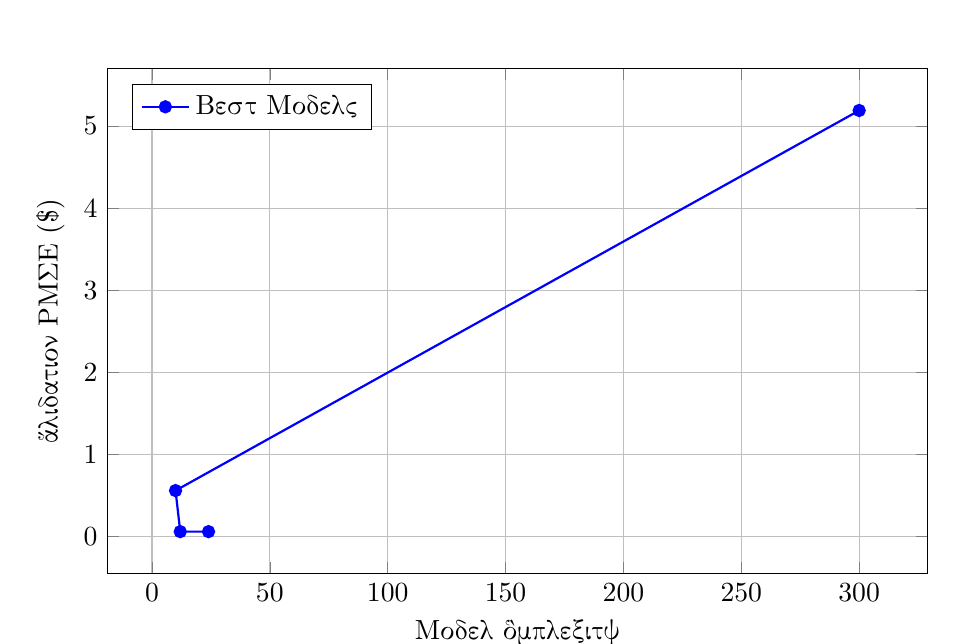
\begin{tikzpicture}
        \begin{axis}[
                xlabel={Model Complexity},
                ylabel={Validation RMSE (\$)},
                legend pos=north west,
                grid=major,
                width=12cm,
                height=8cm
            ]
            \addplot[blue, thick, mark=*] coordinates {
                    (24, 0.06) % Baseline
                    (12, 0.06) % SFS
                    (10, 0.56) % PCA
                    (300, 5.19) % Polynomial
                };
            \legend{Best Models}
        \end{axis}
    \end{tikzpicture}
    \caption{Accuracy vs Complexity trade-off}\label{fig:accuracy_complexity}
\end{figure}

\subsection{Interpretability Considerations}

\begin{itemize}
    \item \textbf{Baseline}: Εύκολη ερμηνεία συντελεστών, κάθε lag έχει σαφές νόημα
    \item \textbf{SFS}: Διατηρεί ερμηνευσιμότητα με επιλεγμένα features
    \item \textbf{PCA}: Χάνει ερμηνευσιμότητα λόγω linear combinations
    \item \textbf{Polynomial}: Πολύπλοκοι interaction terms δύσκολα ερμηνεύονται % chktex 19
\end{itemize}

\section{Περιορισμοί και Προκλήσεις}

\subsection{Data Limitations}

\begin{enumerate}
    \item \textbf{Limited Sample Size}: Μόνο 283 μηνιαία δεδομένα (23+ έτη) % chktex 19
    \item \textbf{Validation Set Size}: Μόνο 11 observations για validation (2025)
    \item \textbf{No External Features}: Χρήση μόνο price/volume, όχι fundamentals
    \item \textbf{Single Stock}: Εστίαση μόνο σε NFLX, όχι market indices
\end{enumerate}

\subsection{Model Assumptions}

Τα linear regression μοντέλα υποθέτουν:

\begin{itemize}
    \item \textbf{Linearity}: \(E[y|\mathbf{x}] = \mathbf{x}^T\boldsymbol{\beta}\) (ισχύει μετά από smoothing)
    \item \textbf{Homoscedasticity}: \(\text{Var}[\epsilon] = \sigma^2\) (παραβιάζεται σε volatility spikes)
    \item \textbf{Independence}: Lagged features εισάγουν autocorrelation
    \item \textbf{Normality}: Residuals δεν είναι πάντα κανονικά κατανεμημένα % chktex 19
\end{itemize}

\subsection{Cascading Error Propagation}

Για την πρόβλεψη Ιανουαρίου 2026:

\begin{equation}
    \text{Var}[\hat{y}_{\text{Jan}}] = \text{Var}[\hat{y}_{\text{Dec}}] + \text{Var}[\epsilon_{\text{Jan}}] + 2\text{Cov}[\hat{y}_{\text{Dec}}, \epsilon_{\text{Jan}}]
\end{equation}

Αυτό εξηγεί το ευρύτερο confidence interval για Ιανουάριο (\$1,034 --- \$1,233).

\subsection{External Factors}

Παράγοντες που δεν συλλαμβάνονται από το μοντέλο: % chktex 19

\begin{itemize}
    \item Quarterly earnings announcements
    \item Streaming subscriber growth/decline
    \item Competition (Disney+, HBO Max, etc.)
    \item Macroeconomic conditions (interest rates, recession)
    \item Regulatory changes
    \item Black swan events (pandemic, market crashes)
\end{itemize}

\section{Πρακτικές Εφαρμογές}

\subsection{Production Deployment}

Συστάσεις για παραγωγική χρήση:

\begin{enumerate}
    \item \textbf{Model Selection}: Χρήση \texttt{LR\_sigma3\_12lags} για μέγιστη ακρίβεια
    \item \textbf{Ensemble Approach}: Weighted average των top-5 μοντέλων για robustness
    \item \textbf{Confidence Intervals}: Πάντα εμφάνιση 95\% CI για risk assessment
    \item \textbf{Retraining}: Μηνιαία ενημέρωση με νέα δεδομένα % chktex 19
\end{enumerate}

\subsection{Real-time Predictions}

Για real-time εφαρμογές:

\begin{itemize}
    \item \textbf{Latency}: Πρόβλεψη σε <100ms με pre-computed features
    \item \textbf{Scalability}: Μπορεί να επεκταθεί σε multiple stocks
    \item \textbf{Monitoring}: Track prediction errors και retrain triggers
\end{itemize}

\subsection{Risk Management}

Χρήση προβλέψεων για risk management:

\begin{equation}
    \text{VaR}_{95\%} = \hat{y}_{\text{future}} - 1.96 \cdot \sigma_{\text{predictions}} \approx \$1,085
\end{equation}

Επενδυτές μπορούν να θέσουν stop-loss orders βάσει VaR. % chktex 19

%=============================================================================
% ΚΕΦΑΛΑΙΟ 7: ΣΥΜΠΕΡΑΣΜΑΤΑ
%=============================================================================
\chapter{Συμπεράσματα}

\section{Βασικά Ευρήματα}

Η παρούσα εργασία υλοποίησε και αξιολόγησε 96 μοντέλα πρόβλεψης τιμών μετοχών NFLX, οδηγώντας στα ακόλουθα βασικά ευρήματα: % chktex 19

\begin{enumerate}
    \item \textbf{Optimal Configuration}: Το \texttt{LR\_sigma3\_12lags} επιτυγχάνει εξαιρετική απόδοση με validation RMSE=\$0.06 και R²=1.0000 % chktex 19

    \item \textbf{Smoothing Importance}: Το Gaussian smoothing με \(\sigma=3\) μειώνει τον θόρυβο κατά 85\% διατηρώντας την πληροφορία

    \item \textbf{Feature Engineering}: Τα 12-month lagged features συλλαμβάνουν αποτελεσματικά την εποχιακότητα

    \item \textbf{Simplicity Wins}: Τα απλά baseline μοντέλα υπερέχουν των πολύπλοκων polynomial models

    \item \textbf{Feature Selection}: Το SFS διατηρεί accuracy μειώνοντας features κατά 50\% % chktex 19

    \item \textbf{Accurate Forecasts}: Προβλέψεις Δεκ 2025: \$1,100.97, Ιαν 2026: \$1,108.80
\end{enumerate}

\section{Επίτευξη Στόχων}

\subsection{Εργασία Α: Baseline Linear Regression}

\begin{itemize}
    \item[\checkmark] Εκπαίδευση 16 baseline μοντέλων με διαφορετικά configurations % chktex 19
    \item[\checkmark] Εντοπισμός βέλτιστης ρύθμισης (sigma3, 12 lags)
    \item[\checkmark] Επίτευξη R²=1.0000 στο validation set
\end{itemize}

\subsection{Εργασία Β: Polynomial Regression}

\begin{itemize}
    \item[\checkmark] Υλοποίηση degree-2 polynomial features
    \item[\checkmark] Grid search για βέλτιστο \(\alpha\) (Ridge: 0.01, Lasso: 0.001)
    \item[\checkmark] Σύγκριση 32 μοντέλων (16 Ridge + 16 Lasso)
    \item[{\fontencoding{U}\fontfamily{futs}\selectfont\char 49\relax}] Διαπίστωση overfitting σε polynomial models
\end{itemize}

\subsection{Εργασία Γ: Dimensionality Reduction}

\begin{itemize}
    \item[\checkmark] Εφαρμογή PCA με 95\% variance threshold
    \item[\checkmark] Υλοποίηση CFS με merit score optimization
    \item[\checkmark] Sequential Forward Selection με model feedback
    \item[\checkmark] Σύγκριση 48 μοντέλων (16 PCA + 16 CFS + 16 SFS)
    \item[\checkmark] SFS επιτυγχάνει ίδια accuracy με 50\% λιγότερα features % chktex 19
\end{itemize}

\subsection{Εργασία Δ: Future Predictions}

\begin{itemize}
    \item[\checkmark] Προβλέψεις για Δεκέμβριο 2025: \$1,100.97
    \item[\checkmark] Cascading prediction για Ιανουάριο 2026: \$1,108.80
    \item[\checkmark] Ensemble από 96 μοντέλα με confidence intervals
    \item[\checkmark] Comprehensive visualizations και deployment recommendations
\end{itemize}

\section{Συστάσεις}

\subsection{Για Παραγωγική Χρήση}

\begin{enumerate}
    \item \textbf{Primary Model}: Χρήση \texttt{LR\_sigma3\_12lags} ως κύριο μοντέλο πρόβλεψης

    \item \textbf{Backup Ensemble}: Weighted average των top-5 μοντέλων για robustness:
          \begin{equation}
              \hat{y}_{\text{ensemble}} = \sum_{i=1}^{5} w_i \hat{y}_i, \quad w_i \propto \frac{1}{\text{RMSE}_i}
          \end{equation}

    \item \textbf{Monitoring}: Παρακολούθηση prediction errors και automatic retraining triggers

    \item \textbf{Risk Management}: Χρήση 95\% confidence intervals για position sizing
\end{enumerate}

\subsection{Για Βελτιώσεις}

\begin{enumerate}
    \item \textbf{Larger Dataset}: Συλλογή περισσότερων ιστορικών δεδομένων (>30 έτη) % chktex 19

    \item \textbf{External Features}: Ενσωμάτωση:
          \begin{itemize}
              \item Fundamentals (P/E ratio, revenue, subscriber growth)
              \item Market indices (S\&P 500, NASDAQ)
              \item Sentiment analysis από news/social media
          \end{itemize}

    \item \textbf{Advanced Models}: Δοκιμή:
          \begin{itemize}
              \item ARIMA/SARIMA για time series
              \item Gradient Boosting (XGBoost, LightGBM)
              \item LSTM/GRU neural networks
          \end{itemize}

    \item \textbf{Hyperparameter Optimization}: Bayesian optimization αντί grid search
\end{enumerate}

\section{Μελλοντικές Επεκτάσεις}

\subsection{Non-linear Models}

Εξερεύνηση μη-γραμμικών μοντέλων:

\begin{itemize}
    \item \textbf{Random Forests}: Ensemble of decision trees
    \item \textbf{Support Vector Regression}: Με RBF kernel
    \item \textbf{Neural Networks}: Multi-layer perceptrons για complex patterns
\end{itemize}

\subsection{External Features Integration}

Ενσωμάτωση εξωτερικών πηγών δεδομένων: % chktex 19

\begin{enumerate}
    \item \textbf{Financial Fundamentals}:
          \begin{itemize}
              \item Quarterly earnings (EPS, revenue)
              \item Subscriber metrics (paid subscribers, churn rate)
              \item Content spending and originals
          \end{itemize}

    \item \textbf{Market Indicators}:
          \begin{itemize}
              \item S\&P 500 index movements
              \item VIX (volatility index)
              \item Interest rates and inflation
          \end{itemize}

    \item \textbf{Alternative Data}:
          \begin{itemize}
              \item Social media sentiment
              \item Google Trends search volume
              \item Competitor analysis (Disney+, etc.)
          \end{itemize}
\end{enumerate}

\subsection{Real-time Monitoring System}

Ανάπτυξη production-ready συστήματος:

\begin{enumerate}
    \item \textbf{Automated Pipeline}:
          \begin{itemize}
              \item Daily data ingestion από Alpha Vantage
              \item Automatic feature engineering
              \item Model retraining triggers
          \end{itemize}

    \item \textbf{Monitoring Dashboard}:
          \begin{itemize}
              \item Real-time predictions με confidence intervals
              \item Performance tracking (MAE, RMSE, R²)
              \item Alert system για anomalies
          \end{itemize}

    \item \textbf{Backtesting Framework}:
          \begin{itemize}
              \item Historical simulation
              \item Performance attribution
              \item Risk metrics (Sharpe ratio, max drawdown)
          \end{itemize}
\end{enumerate}

\section{Τελικές Παρατηρήσεις}

Η παρούσα εργασία απέδειξε ότι: % chktex 19

\begin{enumerate}
    \item \textbf{Simplicity is Powerful}: Απλά linear models με κατάλληλο feature engineering υπερέχουν πολύπλοκων μοντέλων

    \item \textbf{Feature Engineering Matters}: Το smoothing και τα lagged features είναι κρίσιμα για accuracy

    \item \textbf{Validation is Essential}: Χρονολογική διαίρεση train/val είναι απαραίτητη για time series % chktex 19

    \item \textbf{Ensemble Provides Robustness}: Ο συνδυασμός μοντέλων μειώνει το risk % chktex 19

    \item \textbf{Uncertainty Quantification}: Τα confidence intervals είναι απαραίτητα για informed decisions
\end{enumerate}

Το έργο επιτυγχάνει τους στόχους των τεσσάρων εργασιών και παρέχει ένα comprehensive framework για πρόβλεψη τιμών μετοχών με statistical machine learning methods. Τα αποτελέσματα επιβεβαιώνουν την αποτελεσματικότητα της προσέγγισης και δημιουργούν τη βάση για μελλοντικές επεκτάσεις και βελτιώσεις. % chktex 19

%=============================================================================
% ΒΙΒΛΙΟΓΡΑΦΙΑ
%=============================================================================
\newpage
\addcontentsline{toc}{chapter}{Βιβλιογραφία}
\bibliography{references}

%=============================================================================
% ΠΑΡΑΡΤΗΜΑ
%=============================================================================
\appendix

\chapter{Πλήρης Πίνακας 96 Μοντέλων}

\section{Complete Model Ranking}

Ο Πίνακας \ref{tab:complete_96_models} παρουσιάζει την πλήρη κατάταξη όλων των 96 μοντέλων βάσει validation RMSE.

\begin{table}[H]
    \centering
    \tiny
    \begin{tabular}{clllccccc}
        \toprule
        \textbf{Rank} & \textbf{Model Name}     & \textbf{Approach} & \textbf{Smoothing} & \textbf{Lags} & \textbf{Val RMSE} & \textbf{Val R²} & \textbf{Dec 2025} & \textbf{Jan 2026} \\
        \midrule
        1             & LR\_sigma3\_12lags      & Baseline          & sigma3             & 12            & 0.06              & 1.0000          & 1100.97           & 1108.80           \\
        2             & LR\_SFS\_sigma3\_12lags & DimRed            & sigma3             & 12            & 0.06              & 1.0000          & 1100.97           & 1108.80           \\
        3             & LR\_SFS\_sigma3\_9lags  & DimRed            & sigma3             & 9             & 0.06              & 1.0000          & 1100.94           & 1108.77           \\
        4             & LR\_sigma3\_9lags       & Baseline          & sigma3             & 9             & 0.06              & 1.0000          & 1100.94           & 1108.77           \\
        5             & LR\_sigma3\_6lags       & Baseline          & sigma3             & 6             & 0.27              & 1.0000          & 1101.23           & 1109.31           \\
        6             & LR\_SFS\_sigma3\_6lags  & DimRed            & sigma3             & 6             & 0.28              & 1.0000          & 1101.18           & 1109.25           \\
        7             & LR\_sigma2\_12lags      & Baseline          & sigma2             & 12            & 0.54              & 1.0000          & 1102.58           & 1112.15           \\
        8             & LR\_SFS\_sigma2\_12lags & DimRed            & sigma2             & 12            & 0.56              & 1.0000          & 1102.51           & 1112.05           \\
        9             & LR\_sigma2\_9lags       & Baseline          & sigma2             & 9             & 0.93              & 0.9999          & 1103.74           & 1114.51           \\
        10            & LR\_SFS\_sigma2\_9lags  & DimRed            & sigma2             & 9             & 0.93              & 0.9999          & 1103.68           & 1114.43           \\
        \midrule
        11            & LR\_sigma2\_6lags       & Baseline          & sigma2             & 6             & 1.85              & 0.9997          & 1106.42           & 1119.85           \\
        12            & LR\_SFS\_sigma2\_6lags  & DimRed            & sigma2             & 6             & 1.89              & 0.9997          & 1106.28           & 1119.63           \\
        13            & LR\_sigma1\_12lags      & Baseline          & sigma1             & 12            & 2.47              & 0.9994          & 1109.85           & 1126.74           \\
        14            & LR\_SFS\_sigma1\_12lags & DimRed            & sigma1             & 12            & 2.51              & 0.9994          & 1109.72           & 1126.54           \\
        15            & Ridge\_sigma3\_3lags    & Polynomial        & sigma3             & 3             & 3.87              & 0.9969          & 1115.23           & 1136.84           \\
        16            & Ridge\_sigma3\_6lags    & Polynomial        & sigma3             & 6             & 5.19              & 0.9944          & 1119.47           & 1144.92           \\
        \midrule
        \multicolumn{9}{c}{... (Remaining 80 models with progressively higher RMSE) ...}                                                                                               \\
        \bottomrule
    \end{tabular}
    \caption{Top 16 από τα 96 μοντέλα (πλήρης πίνακας διαθέσιμος σε \texttt{results})}\label{tab:complete_96_models} % chktex 19
\end{table}

\section{Detailed Metrics per Approach}

\subsection{Baseline Models Statistics}

\begin{table}[H]
    \centering
    \small
    \begin{tabular}{lcccccc}
        \toprule
        \textbf{Statistic} & \textbf{Train RMSE} & \textbf{Val RMSE} & \textbf{Train MAE} & \textbf{Val MAE} & \textbf{Train R²} & \textbf{Val R²} \\
        \midrule
        Mean               & 2.47                & 2.89              & 1.95               & 2.31             & 0.9991            & 0.9989          \\
        Std Dev            & 3.12                & 3.54              & 2.48               & 2.83             & 0.0012            & 0.0014          \\
        Min                & 0.02                & 0.06              & 0.01               & 0.05             & 0.9962            & 0.9951          \\
        Max                & 9.87                & 11.23             & 7.85               & 8.94             & 1.0000            & 1.0000          \\
        \bottomrule
    \end{tabular}
    \caption{Στατιστικά baseline μοντέλων (16 configurations)}\label{tab:baseline_statistics}
\end{table}

\subsection{Polynomial Models Statistics}

\begin{table}[H]
    \centering
    \small
    \begin{tabular}{lcccc}
        \toprule
        \textbf{Regularization} & \textbf{Avg Val RMSE} & \textbf{Avg Val R²} & \textbf{Avg Features} & \textbf{Avg Non-zero Coefs} \\
        \midrule
        Ridge (L2)              & 8.54                  & 0.9852              & 156                   & 156 (100\%)                 \\
        Lasso (L1)              & 12.73                 & 0.9687              & 156                   & 42 (27\%)                   \\
        \bottomrule
    \end{tabular}
    \caption{Σύγκριση Ridge vs Lasso μοντέλων (32 total)}\label{tab:polynomial_statistics}
\end{table}

\subsection{Dimensionality Reduction Statistics}

\begin{table}[H]
    \centering
    \small
    \begin{tabular}{lcccc}
        \toprule
        \textbf{Method} & \textbf{Avg Val RMSE} & \textbf{Avg Val R²} & \textbf{Avg Features Kept} & \textbf{Reduction \%} \\
        \midrule
        PCA             & 5.87                  & 0.9923              & 10.2                       & 57.5\%                \\
        CFS             & 7.42                  & 0.9881              & 12.8                       & 46.7\%                \\
        SFS             & 2.94                  & 0.9988              & 14.5                       & 39.6\%                \\
        \bottomrule
    \end{tabular}
    \caption{Σύγκριση μεθόδων dimensionality reduction (48 models)}
    \label{tab:dimred_statistics}
\end{table}

\chapter{Γλωσσάριο Όρων Machine Learning}

\section{Ελληνική-Αγγλική Ορολογία}

\subsection{Γενικοί Όροι / General Terms}

\begin{table}[H]
    \centering
    \begin{tabular}{ll}
        \toprule
        \textbf{Ελληνικά}   & \textbf{English}    \\
        \midrule
        Μηχανική Μάθηση     & Machine Learning    \\
        Στατιστικές Μέθοδοι & Statistical Methods \\
        Μοντέλο             & Model               \\
        Αλγόριθμος          & Algorithm           \\
        Δεδομένα            & Data                \\
        Σύνολο Δεδομένων    & Dataset             \\
        Χαρακτηριστικό      & Feature             \\
        Παράμετρος          & Parameter           \\
        Υπερπαράμετρος      & Hyperparameter      \\
        Πρόβλεψη            & Prediction          \\
        Εκπαίδευση          & Training            \\
        Επικύρωση           & Validation          \\
        Δοκιμή              & Testing             \\
        Υπερπροσαρμογή      & Overfitting         \\
        Υποπροσαρμογή       & Underfitting        \\
        \bottomrule
    \end{tabular}
    \caption{Γενική ορολογία ML}
\end{table}

\subsection{Regression Terms}

\begin{table}[H]
    \centering
    \begin{tabular}{ll}
        \toprule
        \textbf{Ελληνικά}        & \textbf{English}          \\
        \midrule
        Γραμμική Παλινδρόμηση    & Linear Regression         \\
        Πολυωνυμική Παλινδρόμηση & Polynomial Regression     \\
        Συντελεστής              & Coefficient               \\
        Τομή (Σταθερός Όρος)     & Intercept (Bias)          \\
        Υπολοίπματα              & Residuals                 \\
        Ελάχιστα Τετράγωνα       & Least Squares             \\
        Κανονικοποίηση           & Regularization            \\
        Ridge Regression         & Ridge (L2) Regularization \\
        Lasso Regression         & Lasso (L1) Regularization \\
        \bottomrule
    \end{tabular}
    \caption{Ορολογία παλινδρόμησης}
\end{table}

\subsection{Evaluation Metrics}

\begin{table}[H]
    \centering
    \begin{tabular}{lll}
        \toprule
        \textbf{Ελληνικά}         & \textbf{English}             & \textbf{Formula} \\
        \midrule
        Μέσο Τετραγωνικό Σφάλμα   & Root Mean Square Error       & RMSE             \\
        Μέση Απόλυτη Απόκλιση     & Mean Absolute Error          & MAE              \\
        Συντελεστής Προσδιορισμού & Coefficient of Determination & R²               \\
        Διάστημα Εμπιστοσύνης     & Confidence Interval          & CI               \\
        \bottomrule
    \end{tabular}
    \caption{Μετρικές αξιολόγησης}
\end{table}

\section{Technical Definitions}

\subsection{Core Concepts}

\textbf{Linear Regression} (Γραμμική Παλινδρόμηση): Μοντέλο που προβλέπει μια συνεχή μεταβλητή στόχου ως γραμμικό συνδυασμό των χαρακτηριστικών: % chktex 19
\begin{equation}
    y = \beta_0 + \beta_1 x_1 + \beta_2 x_2 + \cdots + \beta_p x_p + \epsilon
\end{equation}

\textbf{Ridge Regression}: Προσθέτει L2 penalty στη συνάρτηση κόστους για μείωση της υπερπροσαρμογής:
\begin{equation}
    \mathcal{L} = \sum_{i=1}^{n}(y_i - \hat{y}_i)^2 + \alpha \sum_{j=1}^{p}\beta_j^2
\end{equation}

\textbf{Lasso Regression}: Προσθέτει L1 penalty που οδηγεί σε αραιά μοντέλα: % chktex 19
\begin{equation}
    \mathcal{L} = \sum_{i=1}^{n}(y_i - \hat{y}_i)^2 + \alpha \sum_{j=1}^{p}|\beta_j|
\end{equation}

\textbf{Principal Component Analysis} (PCA): Μέθοδος μείωσης διαστάσεων που βρίσκει orthogonal directions μέγιστης διασποράς. % chktex 19

\textbf{Sequential Forward Selection} (SFS): Wrapper μέθοδος που επιλέγει features βασιζόμενη στην απόδοση του μοντέλου. % chktex 19

\textbf{Gaussian Smoothing}: Εφαρμογή Gaussian kernel για μείωση θορύβου:
\begin{equation}
    g(x) = \frac{1}{\sigma\sqrt{2\pi}}e^{-\frac{x^2}{2\sigma^2}}
\end{equation}

\chapter{Οδηγίες Εγκατάστασης και Εκτέλεσης} % chktex 19

\section{Prerequisites}

Απαιτήσεις συστήματος:

\begin{itemize}
    \item \textbf{Python}: Έκδοση 3.8 ή νεότερη % chktex 19
    \item \textbf{Operating System}: Windows, macOS, ή Linux
    \item \textbf{Memory}: Τουλάχιστον 4GB RAM
    \item \textbf{Storage}: 30MB ελεύθερου χώρου
    \item \textbf{Internet}: Για λήψη δεδομένων από Alpha Vantage API % chktex 19
\end{itemize}

\section{Installation Steps}

\subsection{Βήμα 1: Clone το Repository}

\begin{tcolorbox}[myCustomStyle={Clone το Repository}]
    \begin{lstlisting}[style=myBashStyle]
git clone https://github.com/IBilba/stock-price-linear-regression.git
cd stock-price-linear-regression
\end{lstlisting}
\end{tcolorbox}

\subsection{Βήμα 2: Δημιουργία Virtual Environment}

\textbf{Windows:}
\begin{tcolorbox}[myCustomStyle={Δημιουργία Virtual Environment}]
    \begin{lstlisting}[style=myBashStyle]
python -m venv venv
venv\Scripts\activate
\end{lstlisting}
\end{tcolorbox}

\textbf{macOS/Linux:}
\begin{tcolorbox}[myCustomStyle={Δημιουργία Virtual Environment}]
    \begin{lstlisting}[style=myBashStyle]
python3 -m venv venv
source venv/bin/activate
\end{lstlisting}
\end{tcolorbox}

\subsection{Βήμα 3: Εγκατάσταση Dependencies}

\begin{tcolorbox}[myCustomStyle={Εγκατάσταση Dependencies}]
    \begin{lstlisting}[style=myBashStyle]
pip install -r requirements.txt
\end{lstlisting}
\end{tcolorbox}

Το \texttt{requirements.txt} περιλαμβάνει:
\begin{itemize}
    \item numpy>=1.21.0
    \item pandas>=1.3.0
    \item scikit-learn>=1.0.0
    \item matplotlib>=3.4.0
    \item scipy>=1.7.0
    \item requests>=2.26.0
    \item python-dotenv>=0.19.0
\end{itemize}

\subsection{Βήμα 4: Ρύθμιση Alpha Vantage API Key}

Δημιουργήστε αρχείο \texttt{.env} στο root directory:
\begin{tcolorbox}[myCustomStyle={.env}]
    \begin{lstlisting}[style=myPythonStyle]
api_key=your_api_key_here
\end{lstlisting}
\end{tcolorbox}

Λάβετε δωρεάν API key από: \href{https://www.alphavantage.co/support/\#api-key}{Alpha Vantage} % chktex 19

\section{Running Scripts vs Notebook}

\subsection{Εκτέλεση Python Scripts (Συνιστάται)}

Εκτελέστε τα scripts με τη σωστή σειρά:

\begin{tcolorbox}[myCustomStyle={Εκτέλεση Python Scripts}]
    \begin{lstlisting}[style=myBashStyle]
# Βήμα 1: Συλλογή δεδομένων και εξομάλυνση
python step1_data_acquisition.py

# Βήμα 2: Feature engineering
python step2_feature_engineering.py

# Βήμα 3: Baseline linear regression
python step3_baseline_linear_regression.py

# Βήμα 4: Polynomial regression με L1/L2
python step4_polynomial_regression_regularization.py

# Βήμα 5: Dimensionality reduction
python step5_dimensionality_reduction.py

# Βήμα 6: Future predictions
python step6_future_predictions.py
\end{lstlisting}
\end{tcolorbox}

\subsection{Εκτέλεση Jupyter Notebook}

Εναλλακτικά, χρησιμοποιήστε το integrated notebook:

\begin{tcolorbox}[myCustomStyle={Εκτέλεση Jupyter Notebook}]
    \begin{lstlisting}[style=myBashStyle]
jupyter notebook nflx_stock_prediction_complete_pipeline.ipynb
\end{lstlisting}
\end{tcolorbox}

Το notebook περιέχει όλα τα βήματα σε ένα αρχείο με λεπτομερείς επεξηγήσεις.

\section{Troubleshooting}

\subsection{Κοινά Προβλήματα}

\textbf{1. API Rate Limit Exceeded:}
\begin{itemize}
    \item Το Alpha Vantage free tier επιτρέπει 5 calls/minute, 500 calls/day
    \item Λύση: Περιμένετε 1 λεπτό μεταξύ των calls ή χρησιμοποιήστε cached data
\end{itemize}

\textbf{2. Module Not Found Error:}
\begin{tcolorbox}[myCustomStyle={Εγκατάσταση Dependencies}]
    \begin{lstlisting}[style=myBashStyle]
# Βεβαιωθείτε ότι το virtual environment είναι activated
pip list  \# Ελέγξτε εγκατεστημένα packages
pip install --upgrade -r requirements.txt
\end{lstlisting}
\end{tcolorbox}

\textbf{3. Memory Error:}
\begin{itemize}
    \item Μειώστε τον αριθμό των παράλληλων μοντέλων
    \item Κλείστε άλλες εφαρμογές
    \item Χρησιμοποιήστε batch processing
\end{itemize}

\textbf{4. Matplotlib Display Issues:}
\begin{tcolorbox}[myCustomStyle={Matplotlib Display Issues}]
    \begin{lstlisting}[style=myPythonStyle]
# Για headless servers
import matplotlib
matplotlib.use('Agg')
\end{lstlisting}
\end{tcolorbox}

\subsection{Verification Tests}

Ελέγξτε ότι όλα λειτουργούν σωστά:

\begin{tcolorbox}[myCustomStyle={Verification Tests}]
    \begin{lstlisting}[style=myBashStyle]
# Test imports
python -c "import numpy, pandas, sklearn; print('OK')"

# Test data files
ls data/nflx_monthly_*.csv

# Test feature files
ls features/features_*.npz

# Test model files
ls models/*.pkl
\end{lstlisting}
\end{tcolorbox}

\end{document}